\documentclass[11pt,letter]{article}
\usepackage[top=0.65in,bottom=0.9in,left=0.85in,right=0.85in]{geometry}

%\def\baselinestretch{1.25}
\def\baselinestretch{1.0}

\usepackage[greek, english]{babel}
\usepackage{multicol}

\usepackage[draft]{graphicx}
\usepackage[export]{adjustbox}


% The use of the times package forces the use of the type-1 times
% roman font, but the times roman font does not look nice.
% Besides the times roman font still does not print correctly on
% the dopy printer.
%\usepackage{times}


\usepackage{fancyhdr}
\usepackage{amsmath}
\usepackage{bm}
\usepackage{bbold}
\usepackage{parskip}

\newcommand{\bv}[1]{\ensuremath{\bm{#1}}}
\newcommand{\Lc}{\ensuremath{L_{\mathrm{c}}}}
\newcommand{\dsig}[1]{\ensuremath{ \frac{ d\,\sigma_{#1} }{d\,\Omega} }}

\begin{document}

\section{Scattering of light by an array of atoms}

In our experiment we observe the scattering of photons from atoms confined in
an optical lattice, here we treat this situation by obtaining the the field
scattered from a single atom and then summing the field contributions from all
the atoms coherently at the location of our detector.  The main goal of this
document is to find the connection between the intensity that we measure in our
cameras and the spin structure factor as it is calculated by the theorists in
our collaboration.  

\subsection{Electric field and intensity due to a single atom}

To calculate the scattered field, one uses the source-field expression, which
relates the radiated field to the emitting dipole moment, this is derived in
the standard textbooks~\cite{loudon2000quantum,cohen1998atom}.  The field at
the position of the detector $\bv{r}_{D}$ is given by
\begin{equation} 
    E^{(+)}( \bv{r}_{D}, t) = 
    \eta e^{- i \omega_{L} ( t -r_{D}/c) } 
    S_{-}\left(t - \frac{ r_{D} }{c} \right)
    \label{eq:source-field} 
\end{equation} where $\eta$
is a proportionality factor that we will address later on.  The time-averaged
intensity at the detector is 
\begin{equation}
\label{eq:Idef}
\begin{split}
\langle I (t) \rangle = & 
    \langle E^{(-)}(\bv{r}_{D}, t) E^{(+)}(\bv{r}_{D}, t) \rangle \\
   = & |\eta|^{2} \langle S_{+}(t-r_{D}/c)S_{-}(t-r_{D}/c) \rangle  \\
   = & |\eta|^{2} \langle S_{+}S_{-} \rangle \\
   = & |\eta|^{2} \rho_{ee}  
\end{split} 
\end{equation}
where time dependence is dropped since we are interested in the steady state
solution.  We can write the $S_{\pm}$ operators of the atoms as 
\begin{equation} 
    S_{\pm} = \langle S_{\pm} \rangle + \delta S_{\pm} 
\end{equation}
which defines the difference, $\delta S$, between $S_{\pm}$ and its average
value.   Writing $S_{\pm}$ this way allows us to distinguish between two
components in the radiated light,  the radiation of the average dipole $\langle
S_{\pm}\rangle$ which is the radiation of a classical oscillating dipole with a
phase that is well defined relative to the incident laser field, and the
radiation form the $\delta S_{\pm}$ component which does not have a phase that
is well defined relative to the incident field because it comes form the
fluctuating part of the atomic dipole.  The intensity is then a sum of coherent
and incoherent parts 
\begin{equation} 
I  = \eta^{2} \langle S_{+}\rangle \langle S_{-} \rangle 
   + \eta^{2} \langle \delta S_{+} \delta S_{-} \rangle 
\end{equation}
where we have used the fact that by definition $\langle \delta S_{\pm}
\rangle = 0$. The first and second terms of this equation are the coherent
and incoherent intensity which can be calculated by using the
steady-state solutions to the optical Bloch equations given by
\begin{gather} 
    \langle S_{\pm} \rangle =  u \pm i v  \\
    u =  \frac{ \Delta }{ \Gamma  \sqrt{ I_{\mathrm{p}} / I_{\mathrm{sat}}} } 
         \frac{s}{ 1 + s } \\
    v =  \frac{ 1 } { 2 \sqrt{ I_{\mathrm{p}} / I_{\mathrm{sat}}} } 
         \frac{s}{1+s} \\
\end{gather}
where $s$ is the saturation parameter for an incident probe with intensity
$I_{\mathrm{p}}$:
\begin{equation}
s = \frac{ 2  I_{\mathrm{p}}/I_{\mathrm{sat}} } { 1 + 4(\Delta/\Gamma)^{2} } 
\end{equation}
The coherent and incoherent intensities are
\begin{equation}
\begin{split} 
    \frac{1}{\eta^{2}}  I_{\mathrm{coh}} = &
        \frac{1}{2} \frac{s}{(1+s)^{2} } 
      = \rho_{ee}  \frac{1}{1+s} \\
    \frac{1}{\eta^{2}}  I_{\mathrm{incoh}}  = & 
        \langle S_{+}S_{-} \rangle - \langle S_{+} \rangle \langle S_{-} \rangle
      = \frac{1}{2} \frac{s^{2}}{(1+s)^{2}} = \rho_{ee} \frac{s}{1+s}
 \label{eq:coh-incoh} 
\end{split}
\end{equation}
Note that if we add up coherent and incoherent part we get the more familiar result $I=\eta^{2} \rho_{ee}$, where the total intensity is simply proportional to the population of the excited state.


\subsection{Scattering cross-section}

Now we will turn onto the evaluation of $\eta$, the proportionality factor
between the field and the emitting dipole.  Knowledge of $\eta$ will allow us
to sum coherently the field from a collection of atoms. 

We start by considering the  transition matrix element between the following
initial and final states 
\begin{equation}
\begin{split}
    | \varphi_{i} \rangle = & | g ; \bv{k}\bv{\varepsilon} \rangle \\
    | \varphi_{f} \rangle = & | g ; \bv{k}'\bv{\varepsilon}' \rangle \\
\end{split}
\end{equation}
These states represent the absorption and re-emission of a single photon by the
atom, with two possibly different initial and final photon states.
 
The transition rate to from $i\rightarrow f$ is given by 
\begin{equation}
    \label{eq:transitionRate}
    w_{fi} = \frac{2\pi}{\hbar} | \mathcal{T}_{fi} |^{2} \delta(E_{f}-E_{i})
\end{equation}
Where we use the notation in~\cite{cohen1998atom} (see Exercise~5 on pg. 530),
and $\mathcal{T}_{fi}$ is given by
\begin{equation}
    \mathcal{T}_{fi} = \frac{  
        \langle g; \bv{k}'\bv{\varepsilon}'| H_{I}' | e; 0 \rangle 
        \langle e; 0 | H_{I}' | g; \bv{k}\bv{\varepsilon} \rangle }
        { \hbar\omega - \hbar\omega_{0} + i\hbar (\Gamma/2 ) }
\end{equation} 
where $H_{I}'$ is the interaction Hamiltonian
\begin{equation}
    H_{I}' = -\bv{d} \cdot \bv{E}_{\perp} ( \bv{r} ) 
\end{equation}
and\footnote{Notice that the presence of $\epsilon_{0}$ reveals that we are
using SI units, following the treatment in~\cite{cohen1998atom}.}
\begin{equation}
    \bv{E}_{\perp}(\bv{r}) = i \sum_{j} 
        \left[ \frac{ \hbar \omega_{j} }{ 2\varepsilon_{0} L^{3}}  \right]^{1/2}
        \left( \hat{a}_{j}\bv{\varepsilon}_{j} e^{i\bv{k}_{j}\cdot\bv{r}} 
              - \hat{a}_{j}^{+}\bv{\varepsilon}_{j}^{*} e^{-i\bv{k}_{j}\cdot\bv{r}} 
        \right)
\end{equation}
Using the expressions for $H_{I}'$ and $\bv{E}_{\perp}(\bv{r})$ we obtain for
the matrix element 
\begin{equation}
   \langle e; 0 | H_{I}' | g; \bv{k}\bv{\varepsilon} \rangle = 
       -i \sqrt{ \frac{ \hbar \omega }{2 \varepsilon_{0} L^{3} }} 
      \langle e | (\bv{d} \cdot \bv{\varepsilon}^{*} ) e^{-i\bv{k}\cdot\bv{r}}| g \rangle
\end{equation}
At this point the textbook treatment usually assumes that the atom is at the
origin and that the size of the atom wavefunction is very small compared to
$|\bv{k}|^{-1}$, and so the exponential inside the matrix element typically
does not show up.  In our case the atom is in a lattice site and its center of
mass state is one of the harmonic oscillator states of a lattice well, which,
as we will see, is large enough that the exponential term cannot be neglected.  
 
The states $|e\rangle$ and $|g\rangle$ include the center of mass and internal
states of the atom.  Here we separate the two, and keep the labels $e$, $g$ for
the internal states. Also, we denote the center of mass initial and final
states as $| u \rangle$ and $|u'\rangle$ respectively, and the center of mass
state of the intermediate excited state as $| v\rangle$, we have
\begin{equation}
   \langle e; 0 | H_{I}' | g; \bv{k}\bv{\varepsilon} \rangle = 
       -i \sqrt{ \frac{ \hbar \omega }{2 \varepsilon_{0} L^{3} }} 
      \langle e | \bv{d} \cdot \bv{\varepsilon}^{*} | g \rangle 
      \langle v | e^{-i\bv{k}\cdot\bv{r}} | u \rangle
\end{equation}
and similarly
\begin{equation}
   \langle g; \bv{k}'\bv{\varepsilon}' | H_{I}' | e; 0\rangle = 
       i \sqrt{ \frac{ \hbar \omega' }{2 \varepsilon_{0} L^{3} }} 
      \langle g | \bv{d} \cdot \bv{\varepsilon}' | e \rangle 
      \langle u' | e^{i\bv{k}'\cdot\bv{r}} | v \rangle
\end{equation}
This gives for the matrix element
\begin{equation}
    \mathcal{T}_{fi} = \sum_{v} \frac{\sqrt{\omega \omega'}}{2\varepsilon_{0} L^{3}}
    \frac{ 
      \langle g | \bv{d} \cdot \bv{\varepsilon}' | e \rangle 
      \langle e | \bv{d} \cdot \bv{\varepsilon}^{*} | g \rangle 
      \langle u'| e^{i\bv{k}'\cdot\bv{r}} | v \rangle 
      \langle v | e^{-i\bv{k}\cdot\bv{r}} | u  \rangle
       }
        { \omega - \omega_{0} + i (\Gamma/2 ) }
\end{equation}
where we have summed over all possible intermediate center of mass states.
Note that the sum can be taken out using the closure relation
$\sum_{v}|v\rangle\langle v| = \mathbb{1}$. 
%We note here that the phase factors $i\bv{k}\cdot\bv{r}$ that appear due to
%the center of mass motion of the atom are uncorrelated.   This comes out that
%way because the scattering of a photon is second order: first the photon gets
%absorbed and then it gets reemitted at a later time.   In neutron scattering
%for example, the scattering process is first order, represented by a contact
%interaction between the neutron and the nuclei in the crystal,  In this case
%the phase factor due to the center of mass motion shows up as \begin{equation}
%\langle  e^{i (\bv{k}'-\bv{k}) \cdot \bv{r}} \rangle_{\mathrm{CM}}
%\end{equation} The norm squared of this term is the Debye-Waller factor.   It
%is necessary to consider if the uncorrelated expectation values that appear in
%the second order photon scattering are correct.  To this effect one needs to
%consider the time between absorption and emission processes which is on the
%order of $\Gamma$, the linewidth of the excited state.   This is much larger
%that the typical harmonic oscillator frequency in a lattice site, which is
%about 400 kHz for a lithium atom in a 50 recoil lattice.   With this in mind
%we may think about photon scattering as an effectively first order process
%(scattering and emission happen much quicker than the atom's center of mass
%can move)  and we may take the liberty of writing the transition matrix
%element which includes the center of mass motion as \begin{equation}
%\begin{split} \langle \mathcal{T}_{fi} \rangle_{\mathrm{CM}} = & \left \langle
%\frac{  \langle g; \bv{k}'\bv{\varepsilon}'| H_{I}' | e; 0 \rangle \langle b;
%0 | H_{I}' | g; \bv{k}\bv{\varepsilon} \rangle } { \hbar\omega -
%\hbar\omega_{0} + i\hbar (\Gamma/2 ) } \right \rangle _{\mathrm{CM}} \\ =&
%\frac{\sqrt{\omega \omega'}}{2\varepsilon_{0} L^{3}} \frac{ \langle g | \bv{d}
%\cdot \bv{\varepsilon}' | e \rangle \langle e | \bv{d} \cdot \bv{\varepsilon}
%| g \rangle \langle  e^{i(\bv{k}'-\bv{k}) \cdot\bv{r}} \rangle_{\mathrm{CM}} }
%{ \omega - \omega_{0} + i (\Gamma/2 ) } \end{split} \end{equation} where the
%more famliar Debye-Waller factor shows up.  

In our experiment we are driving a sigma-minus transition so we can consider
only the projection of $\bv{d}$ onto $\bv{\varepsilon}_{-}$ 
\begin{equation}
     \langle e | \bv{d} \cdot \bv{\varepsilon}^{*} | g \rangle  \equiv
     d_{-} (\bv{\varepsilon}_{-}  \cdot \bv{\varepsilon}^{*} )
\end{equation} 
which leads to 
\begin{equation}
    \mathcal{T}_{fi}  = 
    \frac{\sqrt{\omega \omega'}}{2\varepsilon_{0} L^{3}}
    \frac{ |d_{-}|^{2}  (\bv{\varepsilon}_{+}\cdot \bv{\varepsilon}' )
                       (\bv{\varepsilon}^{*}\cdot \bv{\varepsilon}_{-} )}
        { \omega - \omega_{0} + i (\Gamma/2 ) }
      \langle u' | e^{i(\bv{k}'-\bv{k}) \cdot\bv{r}} | u  \rangle
\end{equation}
We use the relation between $|d_{-}|^{2}$ and the linewidth of the transition
\begin{equation} 
    |d_{-}|^{2} =  3\pi \varepsilon_{0} \hbar
  \left( \frac{c}{\omega_{0}} \right)^{3}  \Gamma
\end{equation}
and also the approximation $\omega' \approx \omega \approx \omega_{0}$ for the
square root in the denominator to obtain
\begin{equation}
    \mathcal{T}_{fi} =
    \frac{ 3 } {k^{2}} 
    \frac{ \pi \hbar c } {  L^{3} } 
        (\bv{\varepsilon}_{+}\cdot \bv{\varepsilon}' )
                       (\bv{\varepsilon}^{*}\cdot \bv{\varepsilon}_{-} )
    \frac{ \Gamma/2  }
        { \omega - \omega_{0} + i (\Gamma/2 ) }
      \langle u' | e^{i(\bv{k}'-\bv{k}) \cdot\bv{r}} | u  \rangle
\end{equation}
The number of final states with energy between $\hbar c k'$ and $\hbar c ( k' +
\mathrm{d}k')$  whose wave vector points inside the solid angle $\mathrm{d}
\Omega'$ equals 
\begin{equation}
    \rho( \hbar c k') \hbar c \mathrm{d} k' \mathrm{d} \Omega ' = \frac{L^{3}}{8 \pi^{3} }  k'^{2} \mathrm{d} k' \mathrm{d} \Omega' 
\end{equation}
where $\rho$ is the density of states.  We use this to replace the sum over
$k'$ with an integral,  and obtain the total transition rate 
\begin{equation}
\begin{split}
  \sum_{fu'} w_{fi} = & 
   \frac{2\pi}{\hbar}  \mathrm{d} \Omega' 
      \int_{0}^{\infty} \frac{k'^{2} \mathrm{d} k' }{ (2\pi / L^{3} ) ^{3} } 
   | \mathcal{T}_{fi} |^{2} 
   \delta( \hbar c k' - \hbar c k )  \\ 
   = & 
   \mathrm{d} \Omega' \frac{9}{4 k^{2}} \frac{ c } {L^{3} }
        |(\bv{\varepsilon}_{+}\cdot \bv{\varepsilon}' )
                       (\bv{\varepsilon}^{*}\cdot \bv{\varepsilon}_{-} ) |^{2}
    \left|
    \frac{ \Gamma/2  }
        { \omega - \omega_{0} + i (\Gamma/2 ) }  
      \langle u' | e^{i(\bv{k}'-\bv{k}) \cdot\bv{r}} | u  \rangle
     \right| ^{2} \\ 
   = & 
   \mathrm{d} \Omega' \frac{9}{4 k^{2}} \frac{ c } {L^{3} }
        |(\bv{\varepsilon}_{+}\cdot \bv{\varepsilon}' )
                       (\bv{\varepsilon}^{*}\cdot \bv{\varepsilon}_{-} ) |^{2}
    \frac{ (\Gamma/2)^{2}  }
        { \Delta^{2} +  (\Gamma/2 )^{2} }
    \left|
      \langle u' | e^{i(\bv{k}'-\bv{k}) \cdot\bv{r}} | u  \rangle
\right| ^{2} \\ 
\end{split} 
\end{equation}
If we consider the flux corresponding to the state of the initial photon $\phi
= c/L^{3}$ then we can define the differential cross section 
\begin{equation}
 \frac{ \mathrm{d} \sigma } { \mathrm{d} \Omega'} =  
    \frac{\sum_{f} w_{fi} } { \mathrm{d} \Omega' \phi} = 
    \frac{9}{4 k^{2}} 
        |(\bv{\varepsilon}_{+}\cdot \bv{\varepsilon}' )
                       (\bv{\varepsilon}^{*}\cdot \bv{\varepsilon}_{-} ) |^{2}
    \frac{ (\Gamma/2)^{2}  }
        { \Delta^{2} +  (\Gamma/2 )^{2} }
    \left|
      \langle u' | e^{i(\bv{k}'-\bv{k}) \cdot\bv{r}} | u  \rangle
\right| ^{2}  
\end{equation}
From here we can write down the intensity (of light with polarization
$\bv{\varepsilon}'$) on a detector located at $\bv{r}_{D}$ in the direction of
$\mathrm{d} \Omega'$ as \begin{equation}
\begin{split}
I  =& \frac{1}{r_{D}^{2}} \frac{ \mathrm{d} \sigma } { \mathrm{d} \Omega'}
      I_{\mathrm{p}} 
   =   \frac{1}{r_{D}^{2}} \frac{ \mathrm{d} \sigma } { \mathrm{d} \Omega'}
      \frac{\hbar c k^{3}\Gamma}{6 \pi} \frac{I_{\mathrm{p}}}{I_{\mathrm{sat}}}  \\ 
   =& \frac{\hbar c k \Gamma}{r_{D}^{2}}  
    \frac{9}{4 (6\pi)} 
        |(\bv{\varepsilon}_{+}\cdot \bv{\varepsilon}' )
                       (\bv{\varepsilon}^{*}\cdot \bv{\varepsilon}_{-} ) |^{2}
    \left|
      \langle u' | e^{i(\bv{k}'-\bv{k}) \cdot\bv{r}} | u  \rangle
  \right| ^{2}
     \frac{ I_{\mathrm{probe}} / I_{\mathrm{sat}}}
        { 4(\Delta/\Gamma)^{2} + 1 }
\end{split}
\end{equation}
We identify the last term in the product as $\rho_{ee}$ (in the limit of low
intensity). Comparing with Eq.~\ref{eq:coh-incoh} we can write down an
expression for $\eta$ which was defined back in Eq.~(\ref{eq:Idef}), 
\begin{equation}
  \eta = \left[ \frac{\hbar c k \Gamma}{r_{D}^{2}}  
    \frac{9}{24\pi} \right]^{1/2} 
        (\bv{\varepsilon}_{+}\cdot \bv{\varepsilon}' )
                       (\bv{\varepsilon}^{*}\cdot \bv{\varepsilon}_{-} ) 
      \langle u' | e^{i(\bv{k}'-\bv{k}) \cdot\bv{r}} | u  \rangle
\end{equation}
With an exact expression for $\eta$ we can obtain the field radiated by each
atom and proceed to sum the field coherently for a collection of atoms. 

\subsection{Summation for a collection of atoms} 

For a collection of atoms, the resulting field is the sum of the field produced
by each individual atom, so we have  
\begin{equation}
\begin{split}
\langle I (t) \rangle = & 
    \left\langle \left( \sum_{m} E_{m}^{(-)}(\bv{r}_{D}, t) \right)
            \left( \sum_{n} E_{n}^{(+)}(\bv{r}_{D}, t) \right) \right\rangle \\
\end{split} 
\end{equation}
where we have labeled the atoms with the indices $m$ and $n$.  We insert the
source-field expression from Eq.~\ref{eq:source-field} (dropping the time
dependence) 
\begin{equation}
\begin{split}
 I = &
    \sum_{mn}  \eta_{m}\eta_{n}^{*}  
              \left\langle S_{m+}S_{n-} \right\rangle
\end{split} 
\end{equation}
Using $S=\langle S \rangle + \delta S$, as we did above to obtain the coherent
and incoherent parts of the intensity, we obtain
\begin{equation}
\begin{split}
 I  = &
    \sum_{mn}  \eta_{m}\eta_{n}^{*} \left(
              \langle S_{m+}\rangle \langle S_{n-} \rangle  
            + \langle \delta S_{m+} \delta S_{n-} \rangle \right) \\
    = & 
    \sum_{mn}  \eta_{m}\eta_{n}^{*} 
        \langle  S_{m+}\rangle \langle S_{n-} \rangle 
   + \sum_{n} | \eta_{n}|^{2} \langle \delta S_{n+} \delta S_{n-} \rangle 
\end{split} 
\end{equation}
The steady state solutions of the optical Bloch equations are used again to
evaluate the expectation values and we obtain for $I$
\begin{multline}
 I = 
  \sum_{mn}  \eta_{m}\eta_{n}^{*}
    \left(
    \frac{ \Delta_{m} }{ \Gamma  \sqrt{ I_{\mathrm{p}} / I_{\mathrm{sat}}} } 
    \frac{s_{m}}{ 1 + s_{m} } 
   + i 
    \frac{ 1 } { 2 \sqrt{ I_{\mathrm{p}} / I_{\mathrm{sat}}} } \frac{s_{m}}{1+s_{m}} 
    \right) 
    \left(
    \frac{ \Delta_{n} }{ \Gamma  \sqrt{ I_{\mathrm{p}} / I_{\mathrm{sat}}} } 
    \frac{s_{n}}{ 1 + s_{n} } 
   - i 
    \frac{ 1 } { 2 \sqrt{ I_{\mathrm{p}} / I_{\mathrm{sat}}} } \frac{s_{n}}{1+s_{n}} 
    \right) \\
   + \sum_{n} | \eta_{n}|^{2} \frac{1}{2} \frac{ s_{n}^{2} } { (1 + s _{n} )^{2} } 
\end{multline}
\begin{multline}
 I  = 
  \sum_{mn}  \eta_{m}\eta_{n}^{*}
    \frac{ s_{m} s_{n} } { (I_{\mathrm{p}}/I_{\mathrm{sat}}) ( 1+s_{m} )( 1+s_{n} ) }
    \left(
        \frac{ \Delta_{m} \Delta_{n} }{ \Gamma^{2} } 
      + i \frac{ \Delta_{n} }{ 2 \Gamma } 
      - i \frac{ \Delta_{m} }{ 2 \Gamma } 
      + \frac{1}{4}  
    \right)  
   + \sum_{n} | \eta_{n}|^{2} \frac{1}{2} \frac{ s_{n}^{2} } { (1 + s _{n} )^{2} } 
\end{multline}
The last term here is the incoherently scattered part due to the fluctuating
fraction $\delta S_{\pm}$ of the atomic dipole.  The cross terms do not appear
in this sum because $\langle \delta S_{m+} \delta S_{n-}\rangle =0$ for $m\neq
n$,  this is in fact why this part is identified as the incoherent scattering. 

We proceed to split up the first sum into same-atom ($n=m$) and different atom
($n<m$) parts 
\begin{multline}
 I  = 
  \sum_{m<n} 
    \frac{ s_{m} s_{n} } { (I_{\mathrm{p}}/I_{\mathrm{sat}}) ( 1+s_{m} )( 1+s_{n} ) }
    \left(
        \eta_{m}\eta_{n}^{*}
    \left(
        \frac{ \Delta_{m} \Delta_{n} }{ \Gamma^{2} } 
      + i \frac{ \Delta_{n} }{ 2 \Gamma } 
      - i \frac{ \Delta_{m} }{ 2 \Gamma } 
      + \frac{1}{4}  
    \right)  \right. \\
   \left.  + 
        \eta_{n}\eta_{m}^{*}
    \left(
        \frac{ \Delta_{n} \Delta_{m} }{ \Gamma^{2} } 
      + i \frac{ \Delta_{m} }{ 2 \Gamma } 
      - i \frac{ \Delta_{n} }{ 2 \Gamma } 
      + \frac{1}{4}  
    \right) 
    \right)  \\
  + \sum_{n}  |\eta_{n}|^{2}
    \frac{ s_{n} s_{n} } { (I_{\mathrm{p}}/I_{\mathrm{sat}}) ( 1+s_{n} )( 1+s_{n} ) }
    \left(
        \frac{ \Delta_{n} \Delta_{n} }{ \Gamma^{2} } 
      + \frac{1}{4}  
    \right) \\ 
   + \sum_{n} | \eta_{n}|^{2} \frac{1}{2} \frac{ s_{n}^{2} } { (1 + s _{n} )^{2} } 
\end{multline}

\begin{multline}
 I  = 
  \sum_{m<n} 
    \frac{ s_{m} s_{n} } { (I/I_{\mathrm{sat}}) ( 1+s_{m} )( 1+s_{n} ) }
    2 \Re\left[ 
        \eta_{m}\eta_{n}^{*}
    \left(
        \frac{ \Delta_{m} \Delta_{n} }{ \Gamma^{2} } 
      + i \frac{ \Delta_{n} }{ 2 \Gamma } 
      - i \frac{ \Delta_{m} }{ 2 \Gamma } 
      + \frac{1}{4}  
    \right) \right] \\
  + \sum_{n}  |\eta_{n}|^{2}
    \frac{1}{2}	\frac{ s_{n} } { ( 1+s_{n} )^{2} }
   + \sum_{n} | \eta_{n}|^{2} \frac{1}{2} \frac{ s_{n}^{2} } { (1 + s _{n} )^{2} } 
\end{multline}

With this expression in hand we focus our attention on the terms
$\eta_{m}\eta_{n}^{*}$ and $|\eta_{n}|^{2}$.  We start with the latter 
\begin{equation}
 |\eta_{n}|^{2} =  \frac{\hbar c k \Gamma}{r_{D}^{2}}  
    \frac{9}{24\pi} 
       | (\bv{\varepsilon}_{+}\cdot \bv{\varepsilon}' )
                       (\bv{\varepsilon}^{*}\cdot \bv{\varepsilon}_{-} ) |^{2}
      \langle u | e^{-i(\bv{k}'-\bv{k}) \cdot\bv{r}_{n}} | u'  \rangle
      \langle u' | e^{i(\bv{k}'-\bv{k}) \cdot\bv{r}_{n}} | u  \rangle
\end{equation}
and notice that we have to sum over output polarizations $\bv{\varepsilon}'$
and final center of mass states  $u'$, since our detector does not care about
either. We obtain 
\begin{equation}
\begin{split}
 \sum_{\bv{\varepsilon}' u'}|\eta_{n}|^{2} = & 
    \sum_{ u'} \frac{\hbar c k \Gamma}{r_{D}^{2}}  
    \frac{9}{24\pi} 
      \sum_{\bv{\varepsilon}'} | (\bv{\varepsilon}_{+}\cdot \bv{\varepsilon}' )
                       (\bv{\varepsilon}^{*}\cdot \bv{\varepsilon}_{-} ) |^{2}
      \langle u | e^{-i(\bv{k}'-\bv{k}) \cdot\bv{r}_{n}} | u'  \rangle
      \langle u' | e^{i(\bv{k}'-\bv{k}) \cdot\bv{r}_{n}} | u  \rangle \\
 = & \frac{\hbar c k \Gamma}{r_{D}^{2}}  
    \frac{9}{24\pi} \Lambda 
      \langle u | e^{-i(\bv{k}'-\bv{k}) \cdot\bv{r}_{n}}  e^{i(\bv{k}'-\bv{k}) \cdot\bv{r}_{n}} | u  \rangle \\
 = & \frac{\hbar c k \Gamma}{r_{D}^{2}}  
    \frac{9}{24\pi} \Lambda \\ 
\end{split}
\end{equation}
where we have used the closure relation $\sum{u'}|u'\rangle\langle u'| =
\mathbb{1}$, and have defined for brevity 
\begin{equation}
 \Lambda = 
  \sum_{\bv{\varepsilon}' }
        | (\bv{\varepsilon}_{+}\cdot \bv{\varepsilon}' )
                        (\bv{\varepsilon}\cdot \bv{\varepsilon}_{-} ) |^{2} 
\end{equation} 

Similarly, for $\eta_{m}\eta_{n}^{*}$
\begin{equation}
\begin{split}
 \sum_{\bv{\varepsilon}' u'_{m} u'_{n}} \eta_{m}\eta_{n}^{*} = & 
    \frac{\hbar c k \Gamma}{r_{D}^{2}}  
    \frac{9}{24\pi} \Lambda
 \sum_{u'_{m} u'_{n}} 
      \langle u_{n} | e^{-i(\bv{k}'-\bv{k}) \cdot\bv{r}_{n}} | u'_{n}  \rangle
      \langle u'_{m} | e^{i(\bv{k}'-\bv{k}) \cdot\bv{r}_{m}} | u_{m}  \rangle \\
\end{split}
\end{equation}
In this case we cannot use the closure relation because $n,m$ refer to
different atoms.   We simplify the treatment by considering only final states
for the atom that are the same as the initial state $u'=u$ (these are going to
have the largest matrix elements anyways). In the sum over $u'_{m},u'_{n}$ only
$u'_{m}=u_{m}$ and $u'_{n}=u_{n}$ contribute.  We take the center of mass state
of the atoms to be the ground state of the single lattice site harmonic
oscillator.  This leaves us with 
\begin{equation}
\begin{split}
 \sum_{\bv{\varepsilon}' } \eta_{m}\eta_{n}^{*} = & 
  \frac{\hbar c k \Gamma}{r_{D}^{2}}  
    \frac{9}{24\pi} \Lambda
      \langle 0_{n} | e^{-i(\bv{k}'-\bv{k}) \cdot\bv{r}_{n}} | 0_{n}  \rangle
      \langle 0_{m} | e^{i(\bv{k}'-\bv{k}) \cdot\bv{r}_{m}} | 0_{m}  \rangle \\
\end{split}
\end{equation}

\subsubsection{Debye-Waller factor} 

For each center of mass expectation value we perform a translation $\bv{R}_{n}$
of the coordinate system such that the position of the $n^{\text{th}}$ atom has
a zero expectation value $\langle \bv{r}_{n} \rangle = 0$.  A phase factor
comes out that depends on the position $\bv{R}_{n}$ of the lattice site in
which the atom is located:
\begin{equation}
      \langle 0_{n} | e^{-i(\bv{k}'-\bv{k}) \cdot\bv{r}_{n}} | 0_{n}  \rangle 
    = e^{-i(\bv{k}'-\bv{k}) \cdot\bv{R}_{n}} 
      \langle 0_{n} | e^{-i(\bv{k}'-\bv{k}) \cdot\bv{r}_{n}} | 0_{n}  \rangle
\end{equation} 
We then use the equality $\langle e^{\hat{A}} \rangle = e^{\frac{1}{2} \langle
\hat{A}^{2} \rangle }$, which is valid for a simple harmonic oscillator, where
$\hat{A}$ is any linear combination of displacement and momentum operators of
the oscillator.  This leaves us with
\begin{equation}
\begin{split}
      \langle 0_{n} | e^{-i(\bv{k}'-\bv{k}) \cdot\bv{r}_{n}} | 0_{n}  \rangle 
    = & e^{-i(\bv{k}'-\bv{k}) \cdot\bv{R}_{n}} 
      e^{ -\frac{1}{2} \left\langle 
          [ (\bv{k}'-\bv{k}) \cdot\bv{r}_{n} ]^{2} \right\rangle } \\
    = & e^{ -i \bv{Q} \cdot \bv{R}_{n}} 
      e^{ -\frac{1}{2} \left\langle [ \bv{Q} \cdot\bv{r}_{n} ]^{2} \right\rangle } \\ 
    = & e^{ -i \bv{Q} \cdot \bv{R}_{n}}
      \prod_{i=x,y,z} e^{ - \frac{1}{2}Q_{i}^{2}\langle r_{ni} ^{2} \rangle } \\ 
    = & e^{ -i \bv{Q} \cdot \bv{R}_{n}}
      e^{-W} 
\end{split}
\end{equation} 
where we have defined the momentum transfer $\bv{Q} = \bv{k}' - \bv{k}$,  and
the Debye-Waller factor $e^{-2W}$. 

Putting this back in the expression for $\eta_{m}\eta_{n}^{*}$ we get
\begin{equation}
\begin{split}
 \sum_{\bv{\varepsilon}' } \eta_{m}\eta_{n}^{*} = & 
 \frac{\hbar c k \Gamma}{r_{D}^{2}}  
    \frac{9}{24\pi} \Lambda
       e^{ i \bv{Q}( \bv{R}_{m} - \bv{R}_{n} ) } e^{-2W} 
\end{split}
\end{equation}
And if we now return to the expression for the intensity at the detector we
have 
\begin{multline}
 I  = 
  \sum_{m<n} 
    \frac{ s_{m} s_{n} } 
         { (I_{\mathrm{p}}/I_{\mathrm{sat}}) ( 1+s_{m} )( 1+s_{n} ) }
    2 \Re\left[ 
            \frac{\hbar c k \Gamma}{r_{D}^{2}}  
            \frac{9}{24\pi}  \Lambda
               e^{ i \bv{Q}( \bv{R}_{m} - \bv{R}_{n} ) } e^{-2W}  
    \left(
        \frac{ \Delta_{m} \Delta_{n} }{ \Gamma^{2} } 
      + i \frac{ \Delta_{n} }{ 2 \Gamma } 
      - i \frac{ \Delta_{m} }{ 2 \Gamma } 
      + \frac{1}{4}  
    \right) \right] \\ 
  + \sum_{n}  \frac{1}{2}
    \frac{\hbar c k \Gamma}{r_{D}^{2}}  
    \frac{9}{24\pi} \Lambda
    \frac{ s_{n} } { 1 + s_{n} } 
\end{multline}

\begin{multline}
\label{eq:finalIdetector}
 I  =
 \left( 
 \frac{\hbar c k \Gamma}{r_{D}^{2}}  
     \frac{9}{24\pi} \Lambda 
  \right) \times \\
  \sum_{m<n} 
    \frac{ s_{m} s_{n} } 
         { (I_{\mathrm{p}}/I_{\mathrm{sat}}) ( 1+s_{m} )( 1+s_{n} ) }
    2 \Re\left[ 
               e^{ i \bv{Q}( \bv{R}_{m} - \bv{R}_{n} ) } e^{-2W}  
    \left(
        \frac{ \Delta_{m} \Delta_{n} }{ \Gamma^{2} } 
      + i \frac{ \Delta_{n} }{ 2 \Gamma } 
      - i \frac{ \Delta_{m} }{ 2 \Gamma } 
      + \frac{1}{4}  
    \right) \right]  
  + \sum_{n}  \frac{1}{2}
    \frac{ s_{n} } { 1 + s_{n} } 
\end{multline}
It is good to see that for time-of-flight, where the Debye-Waller factor goes
to zero due to large extent of the expanding atom wavefunctions,  this formula
reduces to the the standard uncorrelated scattering for $N$ atoms with
$\rho_{ee} = \frac{1}{2} \frac{s}{1+s}$.  

{\small
Note:  To see this more clearly and at the same time check the prefactors that show up in this expression, we can evaluate the total photon scattering rate  $\Gamma_{\mathrm{scatt}}= \frac{1}{\hbar c k}\int I r_{D}^{2} \mathrm{d}\Omega $,  for which we use $\int \Lambda \mathrm{d} \Omega = \frac{8\pi}{3}$ to obtain
\begin{equation}
\Gamma_{\mathrm{scatt}} =  \Gamma \frac{1}{2} \frac{s}{1+s} = \Gamma \rho_{ee}
\end{equation} 
 
}


\subsection{ Large detuning limit} 

We start from Eq.~(\ref{eq:finalIdetector}) and concentrate on the two sums,
the first of which is 
\begin{equation} 
  \frac{  e^{-2W}}{2I_{\mathrm{p}}/I_{\mathrm{sat}}} \Re 
  \sum_{m<n} 
               e^{ i \bv{Q}( \bv{R}_{m} - \bv{R}_{n} ) } 
    \frac{ s_{m} s_{n} } {( 1+s_{m} )( 1+s_{n} ) }
    \left(
         4\Delta_{m} \Delta_{n} 
      + 2i \Delta_{n} 
      - 2i \Delta_{m}
      + 1
    \right)  
\end{equation}
where for simplicity we have now written the detunings in units of $\Gamma$.  We will split this up further into four terms 
\begin{align} 
  \frac{  e^{-2W}}{2I_{\mathrm{p}}/I_{\mathrm{sat}}} \Re \sum_{m<n} & 
      e^{ i \bv{Q}( \bv{R}_{m} - \bv{R}_{n} ) } 
      \frac{ s_{m} s_{n} } {( 1+s_{m} )( 1+s_{n} ) } 4 \Delta_{m} \Delta_{n} \\
  \frac{  e^{-2W}}{2I_{\mathrm{p}}/I_{\mathrm{sat}}} \Re \sum_{m<n} & 
      e^{ i \bv{Q}( \bv{R}_{m} - \bv{R}_{n} ) } 
      \frac{ s_{m} s_{n} } {( 1+s_{m} )( 1+s_{n} ) } 2 i \Delta_{n}  \\
  -\frac{  e^{-2W}}{2I_{\mathrm{p}}/I_{\mathrm{sat}}} \Re \sum_{m<n} & 
      e^{ i \bv{Q}( \bv{R}_{m} - \bv{R}_{n} ) } 
      \frac{ s_{m} s_{n} } {( 1+s_{m} )( 1+s_{n} ) } 2 i \Delta_{m}  \\
  \frac{  e^{-2W}}{2I_{\mathrm{p}}/I_{\mathrm{sat}}} \Re \sum_{m<n} & 
      e^{ i \bv{Q}( \bv{R}_{m} - \bv{R}_{n} ) } 
      \frac{ s_{m} s_{n} } {( 1+s_{m} )( 1+s_{n} ) }   
\end{align}

In the low intensity limit, and for a detuning such that $4\Delta_{m}^{2}, 4\Delta_{n}^{2} \gg 1 $ these four tend respectively to 
\begin{align} 
    e^{-2W} 2(I_{\mathrm{p}}/I_{\mathrm{sat}}) \Re \sum_{m<n} & 
      e^{ i \bv{Q}( \bv{R}_{m} - \bv{R}_{n} ) } 
      \frac{1}{ 4 \Delta_{m} \Delta_{n} }  \\
    e^{-2W} 2(I_{\mathrm{p}}/I_{\mathrm{sat}}) \Re \sum_{m<n} & 
      e^{ i \bv{Q}( \bv{R}_{m} - \bv{R}_{n} ) } 
      \frac{i}{ 8 \Delta_{n} \Delta_{m}^{2}} \\
  - e^{-2W} 2(I_{\mathrm{p}}/I_{\mathrm{sat}}) \Re \sum_{m<n} & 
      e^{ i \bv{Q}( \bv{R}_{m} - \bv{R}_{n} ) } 
      \frac{i}{ 8 \Delta_{n}^{2} \Delta_{m} } \\
    e^{-2W} 2(I_{\mathrm{p}}/I_{\mathrm{sat}}) \Re \sum_{m<n} & 
      e^{ i \bv{Q}( \bv{R}_{m} - \bv{R}_{n} ) } 
      \frac{1}{ 16 \Delta_{m}^{2} \Delta_{n}^{2} }
\end{align}
Furthermore, if we detune the light in between the two spin states then we can
use $\frac{1}{2\Delta_{m}} = \frac{1}{|\Delta|}S_{zm}$, where
$S_{zm}=\pm\frac{1}{2}$ is the spin state of the atom in site $m$, to obtain
\begin{align} 
    e^{-2W} \frac{2I_{\mathrm{p}}/I_{\mathrm{sat}}}{ |\Delta|^{2} }  \Re \sum_{m<n} & 
      e^{ i \bv{Q}( \bv{R}_{m} - \bv{R}_{n} ) } 
      S_{zm}S_{zn}  \\
    e^{-2W} \frac{2I_{\mathrm{p}}/I_{\mathrm{sat}}}{ 4 |\Delta|^{3} }  \Re \sum_{m<n} & 
      e^{ i \bv{Q}( \bv{R}_{m} - \bv{R}_{n} ) } 
       i S_{zn} \\
  - e^{-2W} \frac{2I_{\mathrm{p}}/I_{\mathrm{sat}}}{ 4 |\Delta|^{3} }  \Re \sum_{m<n} & 
      e^{ i \bv{Q}( \bv{R}_{m} - \bv{R}_{n} ) }
       i S_{zm} \\  
    e^{-2W} \frac{2I/I_{\mathrm{sat}}}{ 16 |\Delta|^{4} }  \Re \sum_{m<n} & 
      e^{ i \bv{Q}( \bv{R}_{m} - \bv{R}_{n} ) } 
\end{align}
We identify the first term and the last term as related to the spin structure factor and crystal structure factor.
%%%%% that appear in Ted's
%%%%%paper.   We have also two other terms show up here, which Ted discards in his
%%%%%derivation, see more details on Sec.~\ref{sec:Ted}.    As was stated at the
%%%%%beginning of this document, our main goal here is to connect the intensity
%%%%%measured by our cameras with the spin-structure factor that is calculated by the
%%%%%theorists.   
In this last equation we see that the first term, the one related to the spin structure factor, is
going to have the main contribution to the intensity because it goes as $
|\Delta|^{-2} $, whereas the other terms go as larger powers of $1/|\Delta|$.  
If we neglect terms other than the spin structure factor then,  in the low intensity and large detuning limit (with the detuning set in between the two spin states), we obtain 
\begin{equation}
 I  =
 \left( 
 \frac{\hbar c k \Gamma}{r_{D}^{2}}  
     \frac{9}{24\pi} \Lambda 
  \right) \times 
  \left(
    e^{-2W} \frac{2I_{\mathrm{p}}/I_{\mathrm{sat}}}{ |\Delta|^{2} }  \Re \sum_{m<n}  
      e^{ i \bv{Q}( \bv{R}_{m} - \bv{R}_{n} ) } 
      S_{zm}S_{zn}  
  +  \frac{I_{\mathrm{p}}/I_{sat}}{ 4 \Delta^{2} } N
  \right)
\end{equation}
where we have made use of $s_{n}/(1+s_{n}) \approx (I_{\mathrm{p}}/I_{\mathrm{sat}})/ \Delta_{n}^{2}$ to carry out the sum over $n$ in Eq.~(\ref{eq:finalIdetector}).  We then manipulate the $n<m$ sum and the real part to obtain
\begin{equation}
 I  =
 \left( 
 \frac{\hbar c k \Gamma}{r_{D}^{2}}  
     \frac{9}{24\pi} \Lambda 
  \right) \times 
  \left(
    e^{-2W} \frac{I_{\mathrm{p}}/I_{\mathrm{sat}}}{ |\Delta|^{2} }  \sum_{m n}  
      e^{ i \bv{Q}( \bv{R}_{m} - \bv{R}_{n} ) } 
      S_{zm}S_{zn}  
  + (1- e^{-2W}) \frac{I_{\mathrm{p}}/I_{\mathrm{sat}}}{ 4|\Delta|^{2} }  N
  \right)
\end{equation}
In this formula the spin structure factor appears explicitly, we pull out some factors and get  
\begin{equation}
 I  =
 \frac{\hbar c k \Gamma}{r_{D}^{2}}  
     \frac{9}{24\pi} \Lambda
 \frac{I_{\mathrm{p}}/I_{\mathrm{sat}}}{ 4|\Delta|^{2} }  N
  \left(
   1 + 
    e^{-2W} \left( \frac{4}{ N }  \sum_{m n}  
      e^{ i \bv{Q}( \bv{R}_{m} - \bv{R}_{n} ) } 
      S_{zm}S_{zn}  - 1 \right )
     \right)
\end{equation}
After time-of-flight the Debye-Waller factor goes to zero due to the expanding size of the atomic wavefunctions and so  
\begin{equation}
 I_{\mathrm{TOF}} =
 \frac{\hbar c k \Gamma}{r_{D}^{2}}  
     \frac{9}{24\pi} \Lambda
 \frac{I_{\mathrm{p}}/I_{\mathrm{sat}}}{ 4|\Delta|^{2} }  N
\end{equation}
giving finally 
\begin{equation}
 \frac{I}{I_{\mathrm{TOF}}} = 1 +  e^{-2W}( S(\bv{Q}) - 1 )
 \label{eq:lowIntensityBragg} 
\end{equation}
This has the expected form (we got this from David Huse), and it defines the spin structure factor as 
\begin{equation}
    S(\bv{Q}) =  \frac{4}{ N }  \sum_{m n}  
      e^{ i \bv{Q}( \bv{R}_{m} - \bv{R}_{n} ) } 
      S_{zm}S_{zn}  
\end{equation}

IMPORTANT REMARK:   We note here that this derivation which relates the
observed intensity to the spin structure factor relies on the saturation
parameter being much less than 1.   In our case we have
$I_{\mathrm{p}}/I_{\mathrm{sat}}\approx 25$ and $\Delta\approx 6.5$ which gives a saturation
parameter of $s=0.3$ which is less than 1, but maybe not entirely
negligible. We have performed numerical evaluations of the exact
expression for the intensity at the detector which considers saturation
effects to determine what kind of corrections do we need to make to
connect between our measurement and
the exact spin structure factor (more on this below). 

%%%%%\subsection{Walk through Ted's derivation to find missing terms}\label{sec:Ted}
%%%%%
%%%%%We start with Ted's formula for the differential cross section
%%%%%\begin{equation}
%%%%%\begin{split}
%%%%%\dsig{} =& \frac{9}{4k^{2}}
%%%%%              \sum_{\lambda_{f}} | (\bv{e}_{\bv{k}_{f} \lambda_{f}}^{*} \cdot \bv{e}_{m} )
%%%%%                                   (\bv{e}_{m}^{*} \cdot \bv{e}_{\bv{k}_{i} \lambda_{i}}^{*} )
%%%%%                                 |^{2} \\
%%%%%          & \times \sum_{ \sigma,\sigma', j, j' } [ \langle \hat{n}_{j\sigma}\hat{n}_{j'\sigma'}
%%%%%              e^{ i \bv{K} \cdot ( \hat{\bv{r}}_{j} - \hat{\bv{r}}_{j'} ) } \rangle
%%%%%              \bar{f}_{\sigma} {\bar{f}_{\sigma'}}^{*} ]
%%%%%\end{split}
%%%%%\end{equation}
%%%%%and we abbreviate the sum over final polarizations as
%%%%%\begin{equation}
%%%%% \Lambda = \sum_{\lambda_{f}} | (\bv{e}_{\bv{k}_{f} \lambda_{f}}^{*} \cdot \bv{e}_{m} )
%%%%%                                   (\bv{e}_{m}^{*} \cdot \bv{e}_{\bv{k}_{i} \lambda_{i}}^{*} )
%%%%%                                 |^{2}
%%%%%\end{equation}
%%%%%to obtain
%%%%%
%%%%%\begin{equation}
%%%%%\begin{split}
%%%%%\dsig{} =& \frac{9\Lambda}{4k^{2}}
%%%%%               \sum_{ \sigma,\sigma', j, j' } [ \langle \hat{n}_{j\sigma}\hat{n}_{j'\sigma'}
%%%%%              e^{ i \bv{K} \cdot ( \hat{\bv{r}}_{j} - \hat{\bv{r}}_{j'} ) } \rangle
%%%%%              \bar{f}_{\sigma} {\bar{f}_{\sigma'}}^{*} ] \\
%%%%%\end{split}
%%%%%\end{equation}
%%%%%
%%%%%
%%%%%We will begin by disecting the sum that appears in the elastic cross section. The thermal average factorizes and
%%%%%\begin{equation}
%%%%%\begin{split}
%%%%%\langle \hat{n}_{j\sigma}\hat{n}_{j'\sigma'} \rangle = &\, \langle (\frac{1}{2} + \sigma\hat{S}_{zj} )( \frac{1}{2} + \sigma'\hat{S}_{j'} ) \rangle \\
%%%%%       = &\, \frac{1}{4} + \frac{1}{2} \langle \sigma \hat{S}_{zj} \rangle +
%%%%%\frac{1}{2} \langle \sigma'\hat{S}_{zj'} \rangle + \langle \sigma\sigma'\hat{S}_{zj}\hat{S}_{zj'}
%%%%%\rangle \\
%%%%%\end{split}
%%%%%\end{equation}
%%%%%For this last step
%%%%%\begin{center}
%%%%%  \begin{tabular}{ c }
%%%%%    $\hat{n}_{i\uparrow} + \hat{n}_{i\downarrow} = 1$ \\
%%%%%    $\sigma = \pm 1$ \\
%%%%%    $\hat{S}_{zi} = \frac{1}{2}( \hat{n}_{i\uparrow} - \hat{n}_{i\downarrow} )$
%%%%%  \end{tabular}
%%%%%\end{center}
%%%%%We can manually perform the sums over $\sigma\sigma'$ for each of this four terms and define $\alpha$, $\beta$, and $\kappa$,
%%%%%\begin{equation}
%%%%%\begin{split}
%%%%%\frac{1}{4} \sum_{\sigma\sigma'} \bar{f}_{\sigma} \bar{f}_{\sigma'}^{*} = &\,
%%%%%            \frac{1}{4}(\bar{f}_{\uparrow} + \bar{f}_{\downarrow})( \bar{f}_{\uparrow}^{*} + \bar{f}_{\downarrow}^{*} ) \\
%%%%%       =&\, \frac{1}{4} | \bar{f}_{\uparrow} + \bar{f}_{\downarrow} | ^{2} \equiv \alpha
%%%%%\end{split}
%%%%%\end{equation}
%%%%%
%%%%%\begin{equation}
%%%%%\begin{split}
%%%%%\frac{1}{2} \sum_{\sigma\sigma'} \sigma'\bar{f}_{\sigma} \bar{f}_{\sigma'}^{*} = &\,
%%%%%  \frac{1}{2} (
%%%%%            - \bar{f}_{\downarrow}\bar{f}_{\downarrow}^{*}
%%%%%            + \bar{f}_{\downarrow}\bar{f}_{\uparrow}^{*}
%%%%%            - \bar{f}_{\uparrow}\bar{f}_{\downarrow}^{*}
%%%%%            + \bar{f}_{\uparrow}\bar{f}_{\uparrow}^{*} ) \equiv \kappa
%%%%%\end{split}
%%%%%\end{equation}
%%%%%
%%%%%\begin{equation}
%%%%%\begin{split}
%%%%%\frac{1}{2} \sum_{\sigma\sigma'} \sigma \bar{f}_{\sigma} \bar{f}_{\sigma'}^{*} = &\,
%%%%%  \frac{1}{2} (
%%%%%            - \bar{f}_{\downarrow}\bar{f}_{\downarrow}^{*}
%%%%%            - \bar{f}_{\downarrow}\bar{f}_{\uparrow}^{*}
%%%%%            + \bar{f}_{\uparrow}\bar{f}_{\downarrow}^{*}
%%%%%            + \bar{f}_{\uparrow}\bar{f}_{\uparrow}^{*} ) \equiv \kappa^{*}
%%%%%\end{split}
%%%%%\end{equation}
%%%%%
%%%%%\begin{equation}
%%%%%\begin{split}
%%%%%\sum_{\sigma\sigma'} \sigma\sigma' \bar{f}_{\sigma} \bar{f}_{\sigma'}^{*} = &\,
%%%%%            (\bar{f}_{\uparrow} + \bar{f}_{\downarrow})( \bar{f}_{\uparrow}^{*} + \bar{f}_{\downarrow}^{*} ) \\
%%%%%       =&\, | \bar{f}_{\uparrow} - \bar{f}_{\downarrow} | ^{2} \equiv \beta
%%%%%\end{split}
%%%%%\end{equation}
%%%%%
%%%%%The elastic cross section is then
%%%%%\begin{equation}
%%%%%\begin{split}
%%%%%\dsig{E} =& \frac{9\Lambda}{4k^{2}}
%%%%%               \sum_{ j j' } \langle
%%%%%              e^{ i \bv{K} \cdot ( \hat{\bv{r}}_{j} - \hat{\bv{r}}_{j'} ) } \rangle
%%%%%             \left( \alpha + \langle \hat{S}_{zj}\rangle \kappa + \langle \hat{S}_{zj'} \rangle \kappa^{*}
%%%%%                     + \langle \hat{S}_{zj} \hat{S}_{zj'} \rangle \beta \right)
%%%%%\end{split}
%%%%%\end{equation}
%%%%%
%%%%%In the Bragg scattering paper by Ted, the two central terms are ignored, but there is no mention of why they are ignored.  As we saw above they also appear in the treatement of scattering that we have undertaken here.  
%%%%%

\section{Numerical evaluation of the scattered intensity}


For the numerical calculation we start from Eq.~(\ref{eq:finalIdetector}) and replace the sum over $m<n$ with an unrestricted sum over $m,n$.  This removes the real part, and we have to subtract again some $m=n$ terms, the result is 
\begin{multline}
 I  =
 \left( 
 \frac{\hbar c k \Gamma}{r_{D}^{2}}  
     \frac{9}{24\pi} \Lambda 
  \right) \times \\
  \frac{ e^{-2W} }{ 4 (I_{\mathrm{p}}/I_{\mathrm{sat}})} \sum_{mn} 
    \frac{ s_{m} s_{n} } { ( 1+s_{m} )( 1+s_{n} ) }
               e^{ i \bv{Q}( \bv{R}_{m} - \bv{R}_{n} ) }
    \left(
        4 \Delta_{m} \Delta_{n}
      + 2 i \Delta_{n} 
      - 2 i \Delta_{m}
      + 1
    \right)  
  + \sum_{n}  \frac{1}{2}
    \frac{ s_{n} } { 1 + s_{n} } \left( 1 - \frac{e^{-2W}}{1+s_{n}} \right)
\end{multline}
We will split this up as 
\begin{multline}
 I  =
 \left( 
 \frac{\hbar c k \Gamma}{r_{D}^{2}}  
     \frac{9}{24\pi} \Lambda 
  \right) \times \\
  \left[
  \frac{ e^{-2W} }{ 4 (I_{\mathrm{p}}/I_{\mathrm{sat}})}
  \left( 
    2 \sum_{m}  
    \frac{ s_{m} }
         {  1 + s_{m} } \Delta_{m} e^{i\bv{Q}\cdot\bv{R}_{m} }
    2 \sum_{n} 
    \frac{ s_{n} }
         {  1 + s_{n} } \Delta_{n} e^{-i\bv{Q}\cdot\bv{R}_{n} }  \right. \right.\\
    + 2i\sum_{m}  
    \frac{ s_{m} }
         {  1 + s_{m} } e^{i\bv{Q}\cdot\bv{R}_{m} }
    \sum_{n} 
    \frac{ s_{n} }
         {  1 + s_{n} } \Delta_{n} e^{-i\bv{Q}\cdot\bv{R}_{n} }   \\
    - 2i\sum_{m}  
    \frac{ s_{m} }
         {  1 + s_{m} } \Delta_{m} e^{i\bv{Q}\cdot\bv{R}_{m} }
    \sum_{n} 
    \frac{ s_{n} }
         {  1 + s_{n} } e^{-i\bv{Q}\cdot\bv{R}_{n} }   \\
    \left.
    +\sum_{m}  
    \frac{ s_{m} }
         {  1 + s_{m} } e^{i\bv{Q}\cdot\bv{R}_{m} }
    \sum_{n} 
    \frac{ s_{n} }
         {  1 + s_{n} } e^{-i\bv{Q}\cdot\bv{R}_{n} }  \right) \\
   \left.
  + \sum_{n}  \frac{1}{2}
    \frac{ s_{n} } { 1 + s_{n} } \left( 1 - \frac{e^{-2W}}{1+s_{n}} \right) \right]
\end{multline}
The following sums appear and we define some shorthand notation for them
\begin{align} 
     \Phi \equiv & 
     \sum_{m}  
    \frac{ s_{m} }
         {  1 + s_{m} } \Delta_{m} e^{i\bv{Q}\cdot\bv{R}_{m} } \\
     \Upsilon \equiv &
     \sum_{m}  
    \frac{ s_{m} }
         {  1 + s_{m} } e^{i\bv{Q}\cdot\bv{R}_{m} } \\
     \kappa \equiv & 
     \sum_{n}  
     \frac{ s_{n} } { 1 + s_{n} }  \\
     \xi \equiv & 
     \sum_{n}  
     \frac{ s_{n} } { (1 + s_{n})^{2}}  \\
\end{align}
We can then write the intensity as 
\begin{equation}
\begin{split}
 I  = &
 \left( 
 \frac{\hbar c k \Gamma}{r_{D}^{2}}  
     \frac{9}{24\pi} \Lambda 
  \right)
  \left[
  \frac{ e^{-2W} }{ 4 (I_{\mathrm{p}}/I_{\mathrm{sat}})}
  \left( 
    4 \Phi \Phi^{*}
    + 2i \Upsilon \Phi^{*} 
    - 2i \Phi \Upsilon^{*}
    + \Upsilon \Upsilon^{*}  
          \right)
  + \frac{1}{2}\kappa - \frac{ e^{-2W}}{2} \xi
\right] \\ 
\end{split}
\end{equation}
For the numerical evaluation we will use $\frac{\hbar c k \Gamma}{r_{D}^{2}}  
     \frac{9}{48\pi}$  as a unit for the intensity, so we can finally simplify the expression to
\begin{equation}
\begin{split}
  I  = &
 \Lambda 
  \left[
  \kappa + 
  e^{-2W} \left(  
  \frac{ | \Upsilon - 2 i \Phi |^{2} }{  2 (I_{\mathrm{p}}/I_{\mathrm{sat}})}
   - \xi \right)
  \right] \\ 
\end{split}
\end{equation}
We recall that 
\begin{equation}
 \Lambda = 
  \sum_{\bv{\varepsilon}' }
        | (\bv{\varepsilon}_{+}\cdot \bv{\varepsilon}' )
                        (\bv{\varepsilon}\cdot \bv{\varepsilon}_{-} ) |^{2} 
\end{equation} 

\subsection{Evaluation in a lattice with AFM core and random shell}

For the numerical evaluation of the scattered intensity we will consider a
lattice with $L\times L\times L$ sites in which there is a core of size
$L_{\mathrm{AFM}} \times L_{\mathrm{AFM}} \times L_{\mathrm{AFM}}$ in which the
atoms have antiferromagnetically ordered spins.   The distribution of the spins
outside the core is random, but the spin imbalance is constrained to be zero,
so there is an equal number of atoms in state $|1\rangle$ and state
$|2\rangle $  occupying the $L^{3}$ sites in the lattice.

\subsubsection{Available values of momentum transfer $\bv{Q}$}

In our experiment we sample four different values of the momentum
transfer vector $\bv{Q}$ by sending the probe beam in from different
viewports in our vacuum chamber.   A schematic of this is shown in Fig.~\ref{fig:bragg_scattering_setup}. 
\begin{figure}
\centering 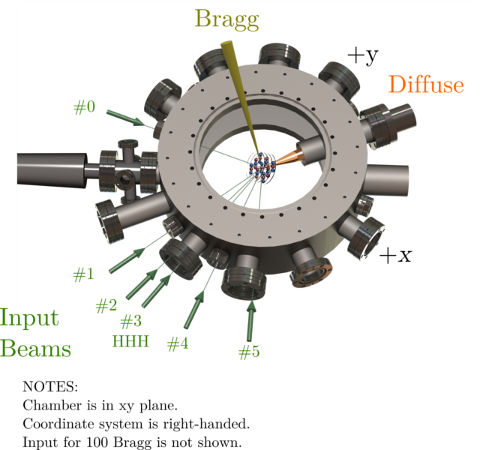
\includegraphics[width=0.75\textwidth]{figures/bragg_setup_illustration_320px.png}
\caption[Bragg scattering setup]{\small Figure shows the different input directions that allow us to measure the spin structure factor at various values of the momentum transfer $\bv{Q}$.  }
\label{fig:bragg_scattering_setup}
\end{figure}

\subsubsection{Debye-Waller factor} 

We will start by showing plots of the Debye-Waller factor as a function of time-of-flight and lattice depth for some of the momentum transfer values.  Plots are as a function of lattice depth (Fig.~\ref{fig:debye-waller_HHH_v0}) and also time-of-flight for a 20 recoil lattice (Fig.~\ref{fig:debye-waller_HHH_tof}).
\begin{figure}
\centering 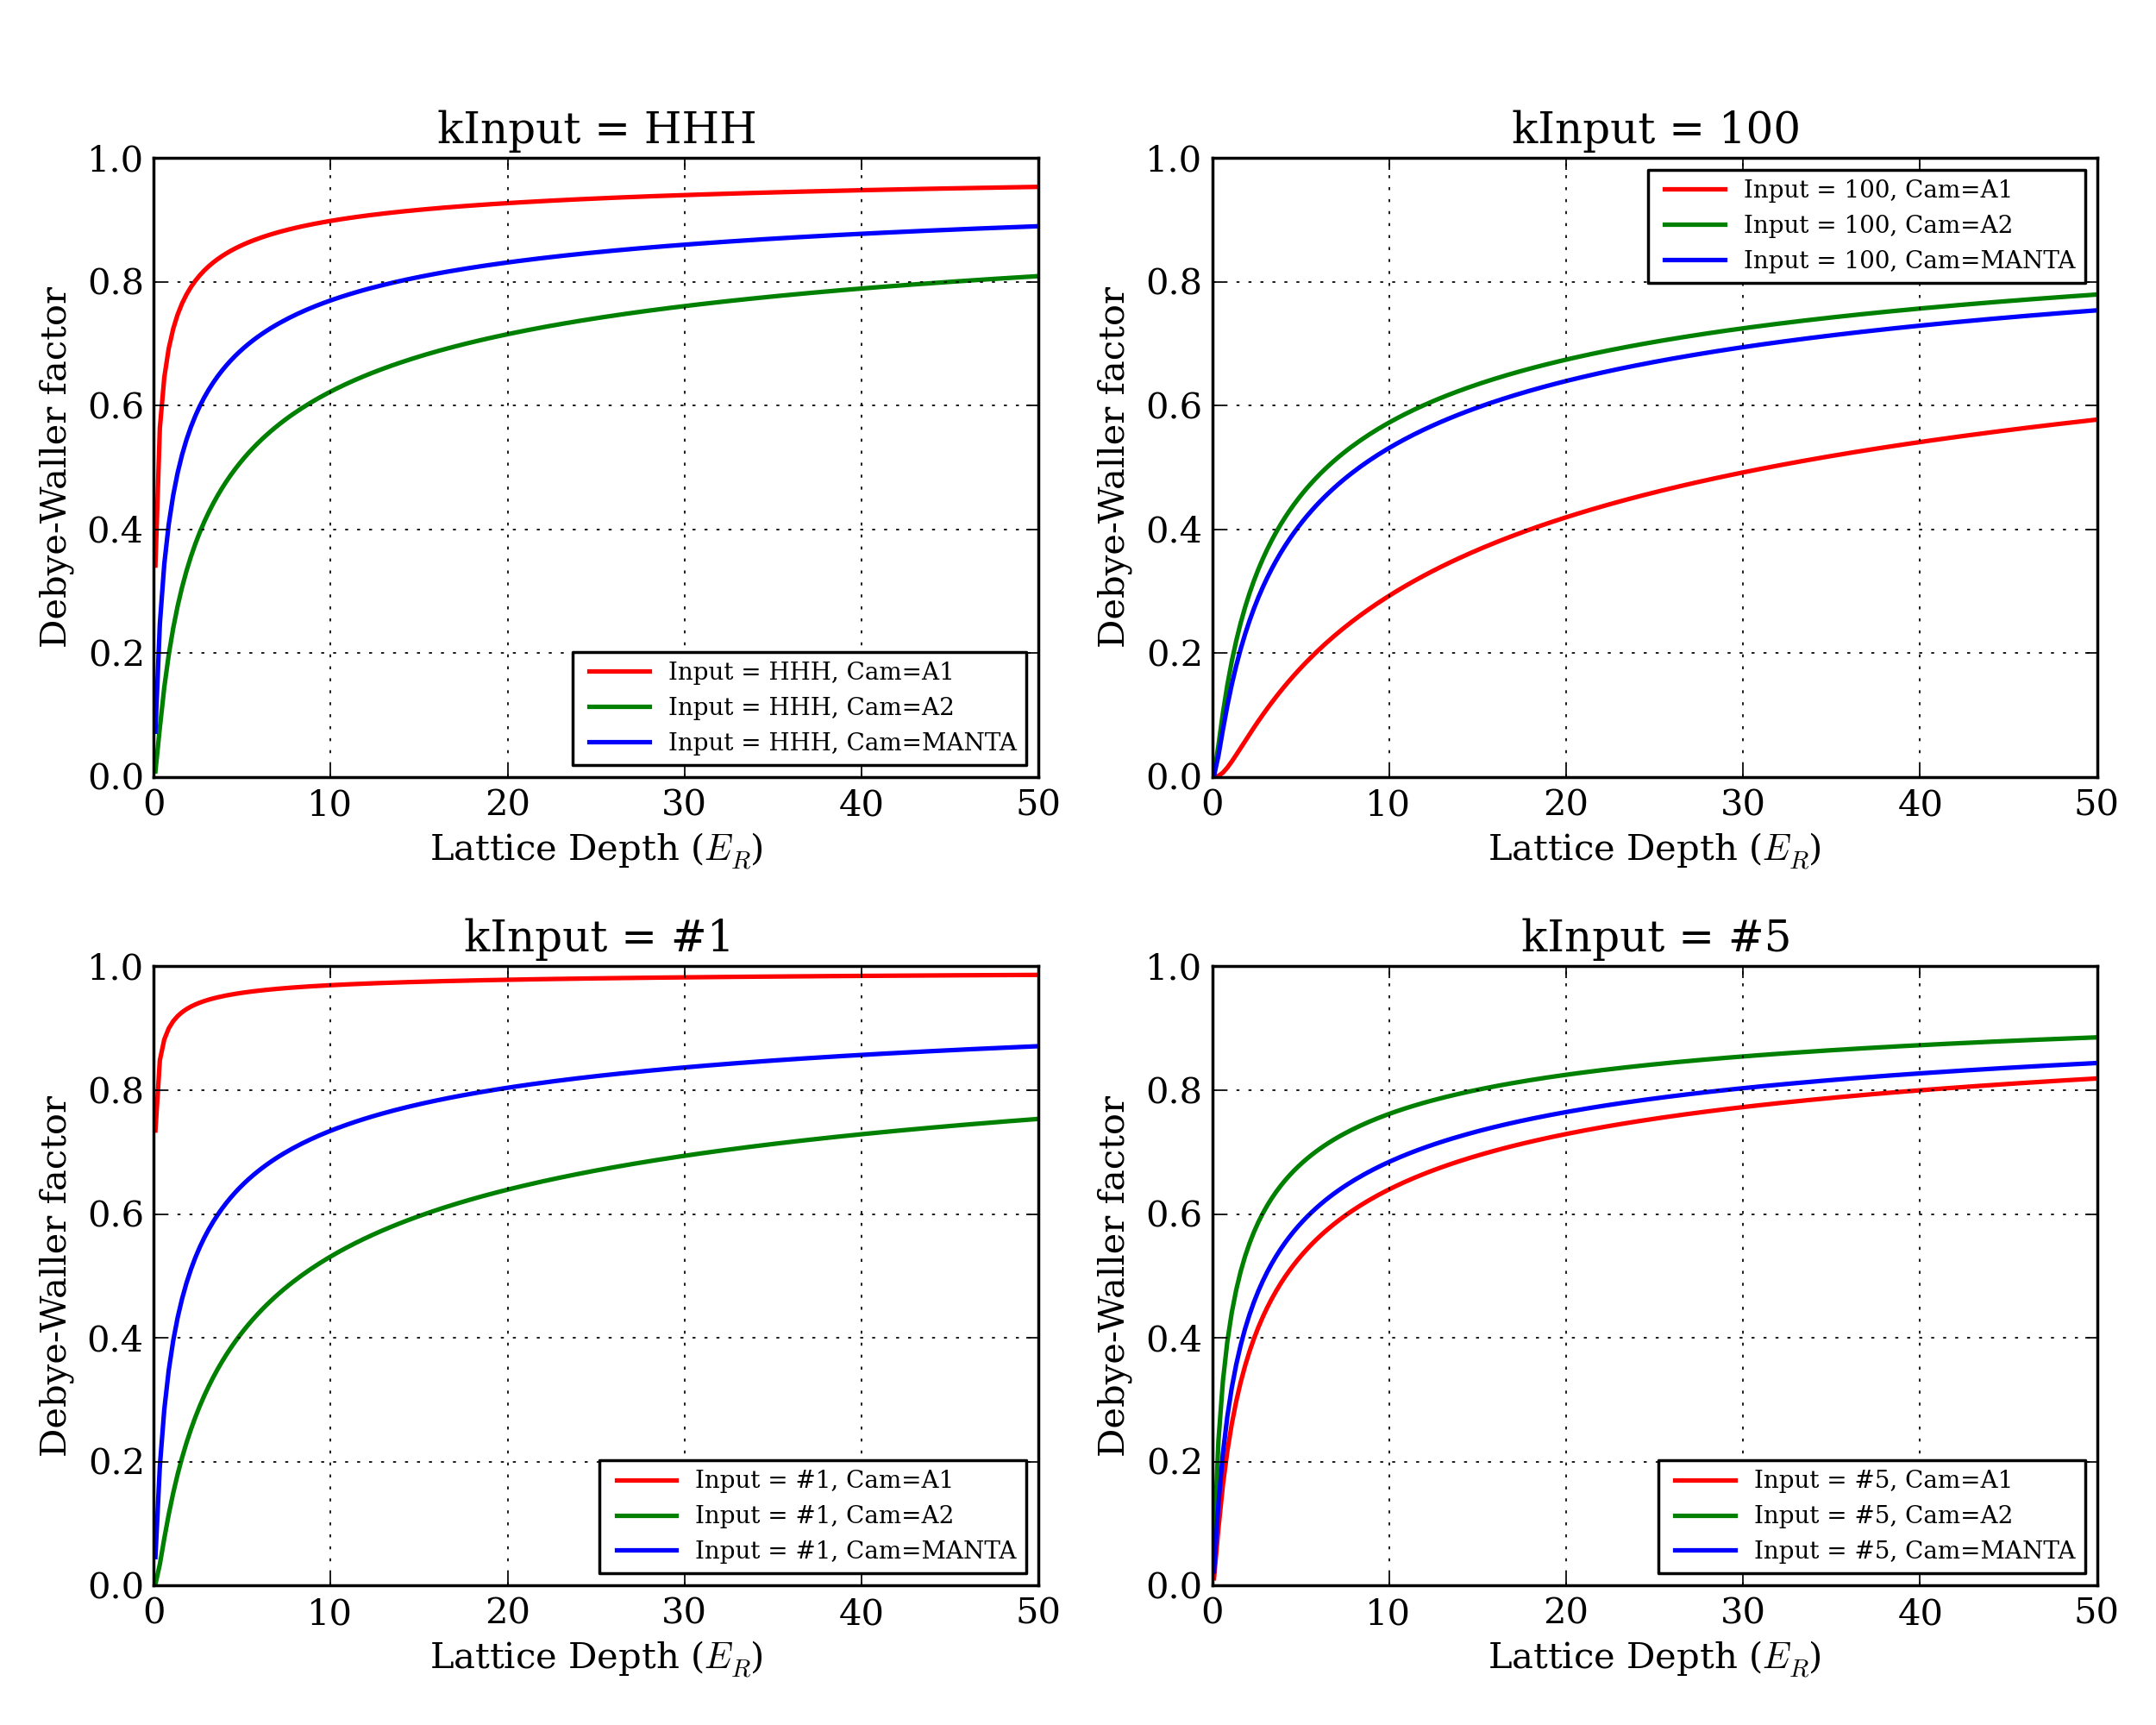
\includegraphics[width=\textwidth]{../debye-waller_HHH/DWv0_plot.png}
\caption[Debye-Waller vs. Lattice depth]{\small Figure shows the Debye-Waller factor as a function of lattice depth for different momentum transfers.}
\label{fig:debye-waller_HHH_v0}
\end{figure}
\begin{figure}
\centering 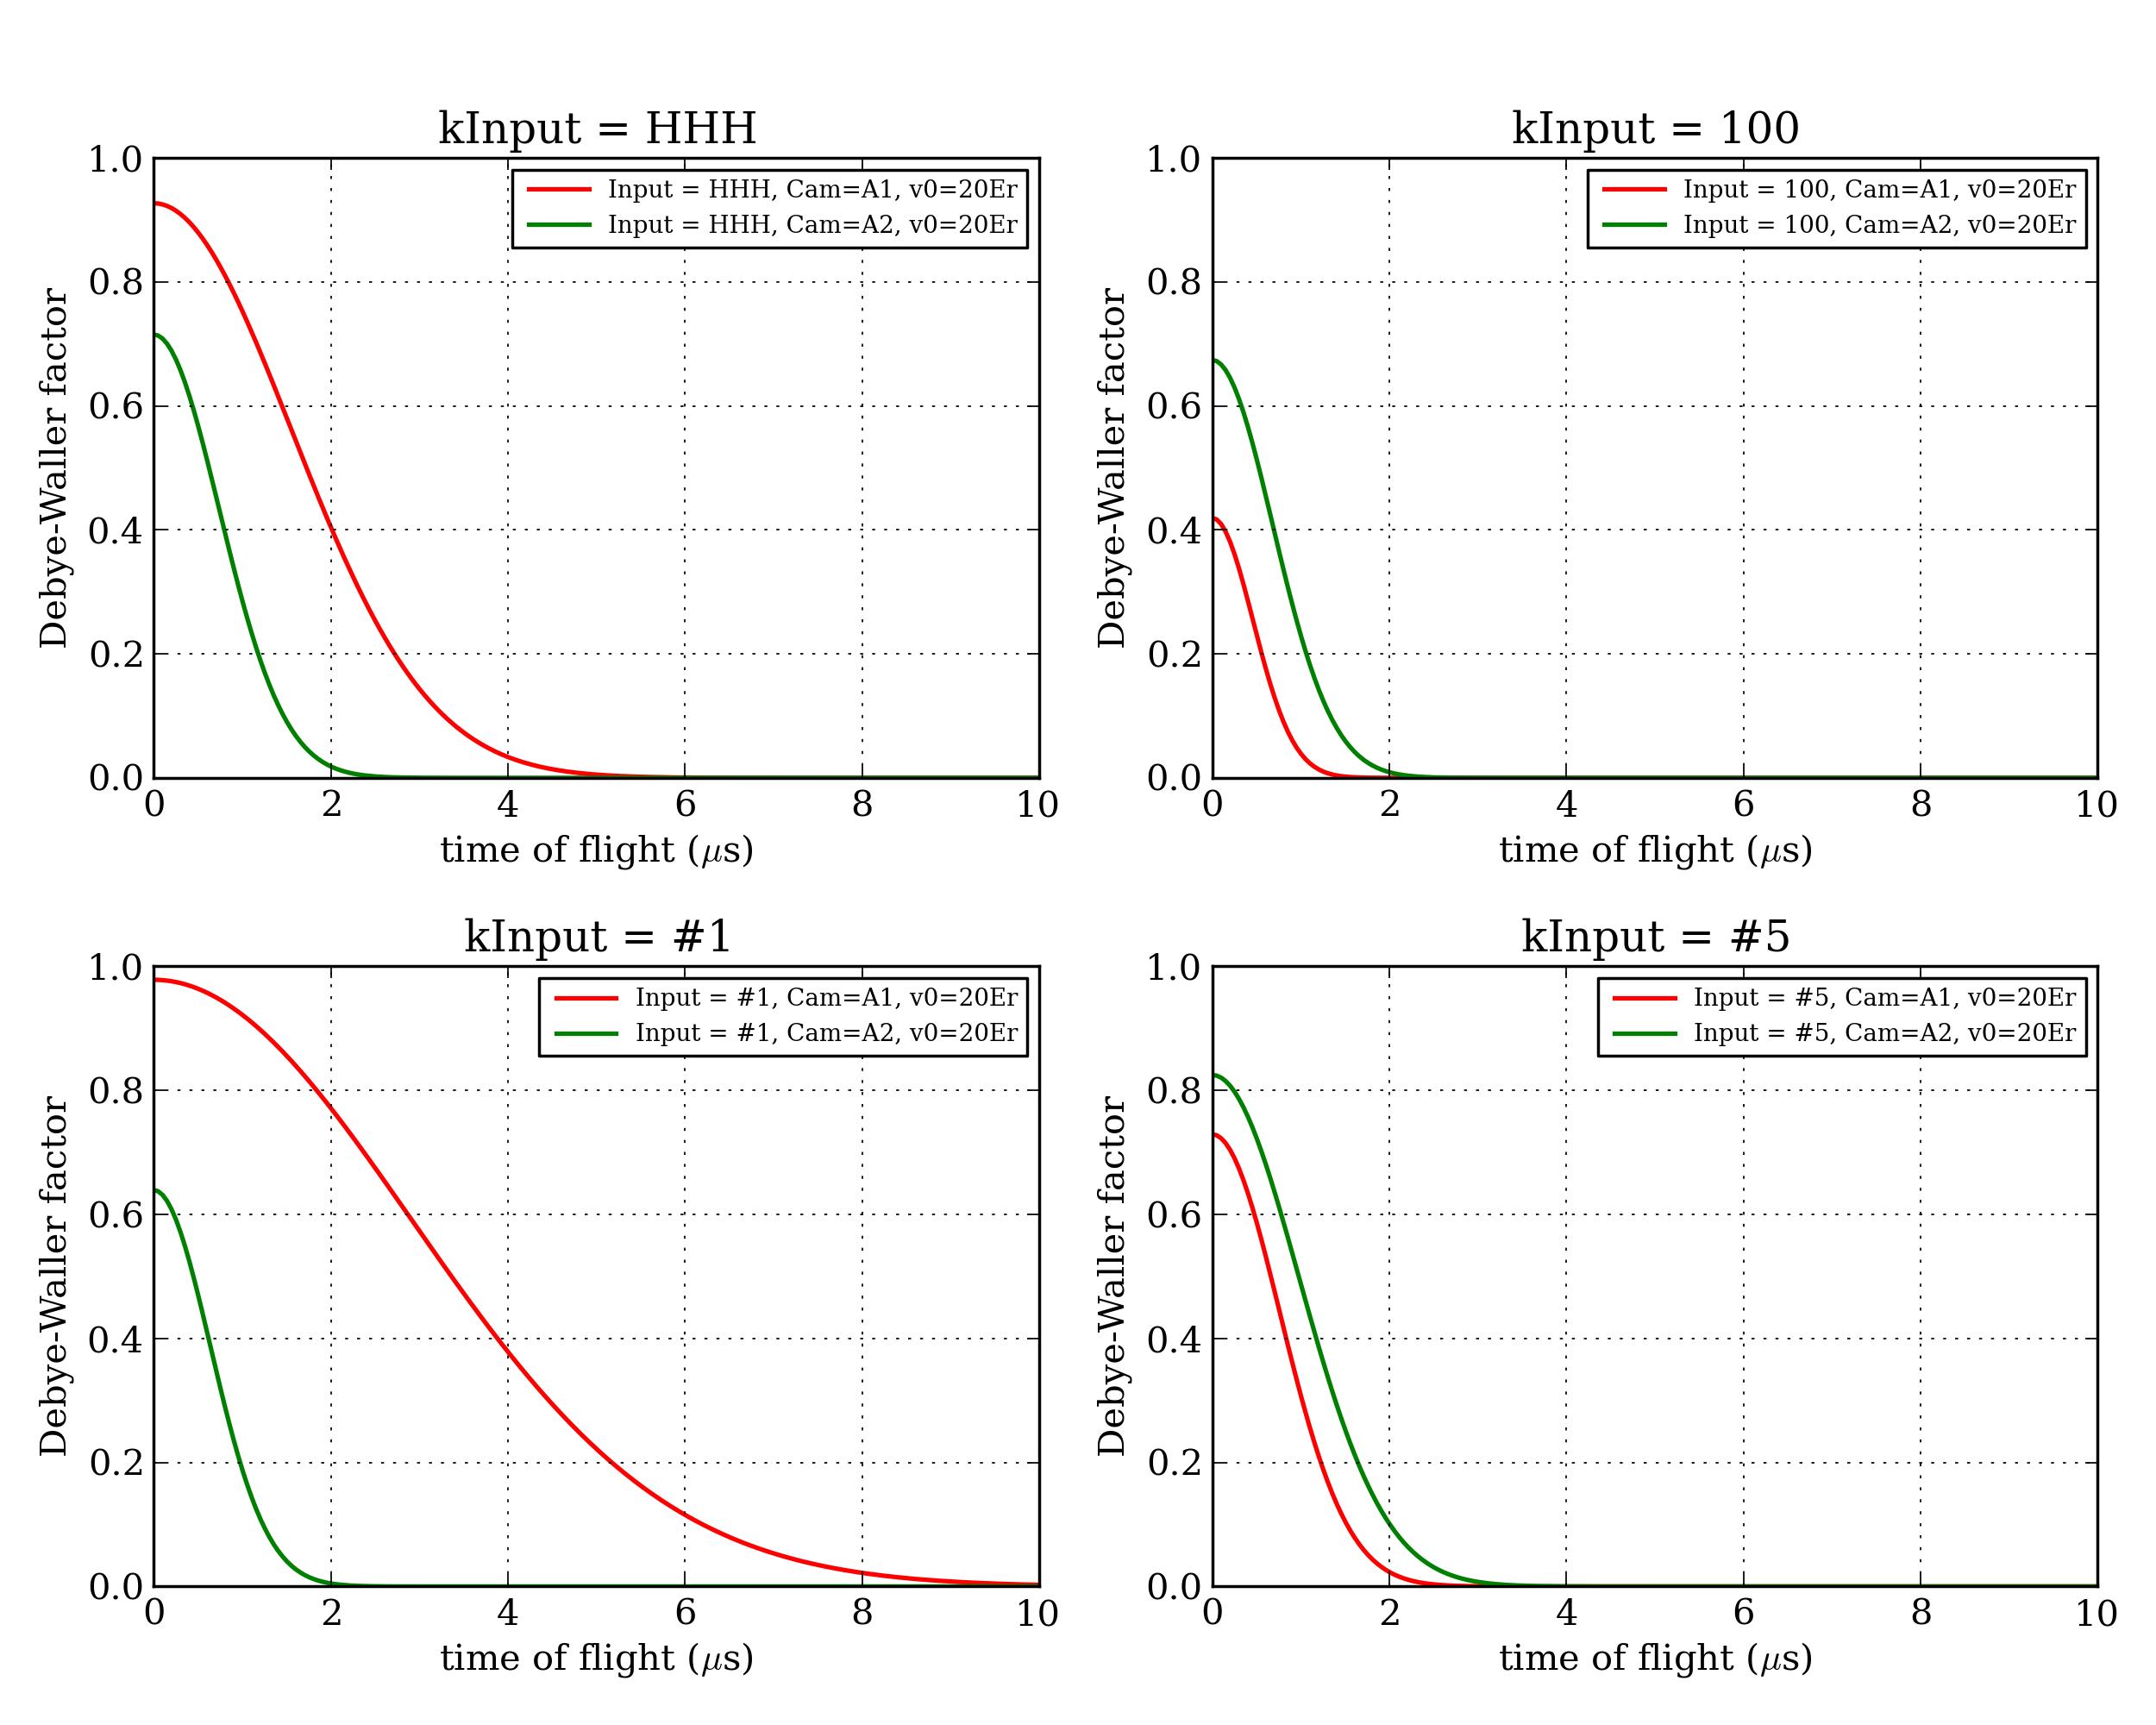
\includegraphics[width=\textwidth]{../debye-waller_HHH/DWtof_plot_20Er.png}
\caption[Debye-Waller vs. TOF]{\small Figure shows the Debye-Waller factor as a function of TOF for different momentum transfers. At $t=0$ the atoms are released from a 20 recoil lattice.}
\label{fig:debye-waller_HHH_tof}
\end{figure}

\subsubsection{Saturation due to probe intensity} 

We look at the saturation due to the probe intensity for a momentum transfer $\bv{Q}_{\mathrm{AF}}$ corresponding to the HHH Bragg scattering peak for antiferromagnetically ordered sample, see Fig.~\ref{fig:pbragg_HHH}. 
\begin{figure}:
\centering 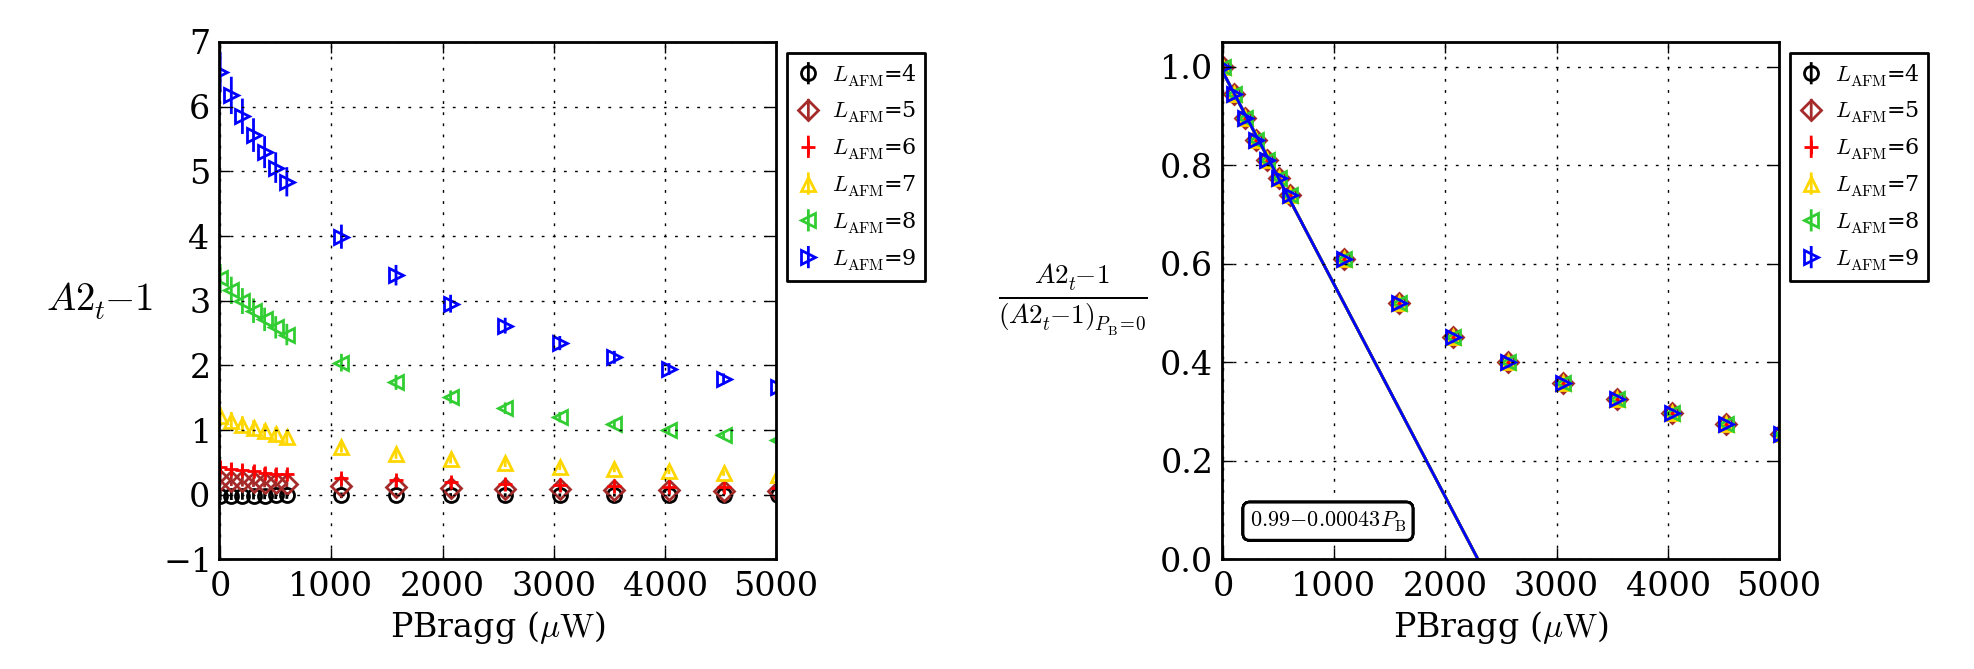
\includegraphics[width=\textwidth]{../pbragg_HHH/pbragg_HHH.png}
\caption[Bragg vs. Power]{\small We use the abbreviation $\frac{X}{X_{\mathrm{TOF}}}=X_{t}$. Left panel shows the Bragg scattering
intensity at camera $A2$ for a beam on the HHH input (Input \#3) as a
function of probe power (Power translates into intensity given the known
beam waist at the atoms). This corresponds to a momentum transfer equal
to $\bv{Q}_{\mathrm{AF}}$.  The various sets correspond to different
sizes of the AFM core used in the numerical evaluation.   Right panel
shows the same as the left panel, but normalized to the value at zero
power for each set.  All the sets collapse into one, and the dependency due to power at low powers is fitted to a straight line.} \label{fig:pbragg_HHH}
\end{figure}
In this case we find that for the power that we are using, $\approx 250
\,\mu\mathrm{W}$,  the excess of counts at the Bragg camera $A2$, for an
in-situ picture with respect to a TOF picture, are underestimated by $\approx$11\%.   

At the moment we will carry on with the assumption that our measurement
is in the low intensity regime, in this case we can go by
Eq.~(\ref{eq:lowIntensityBragg}) to get the value of the spin structure
factor since we know the value of the Debye-Waller factors for each of
the momentum transfers that we measure.  Due to saturation effects then our value can be thought of as a lower bound to $S(\bv{Q})$.  In the future we are going to try to repeat the measurements with a lower Bragg power so that we do not run into this kind of issues.   

\subsection{Estimating the size of the AFM domain}

In our numerical evaluation of the scattered intensity we consider a lattice
with an AFM domain in the center surrounded by a core with a random spin
distribution.   This allows us to study the effect of the outside shell on our
ability to see an AFM distribution in the core, see
Fig.\ref{fig:braggCrystalSize}.
\begin{figure}
\centering 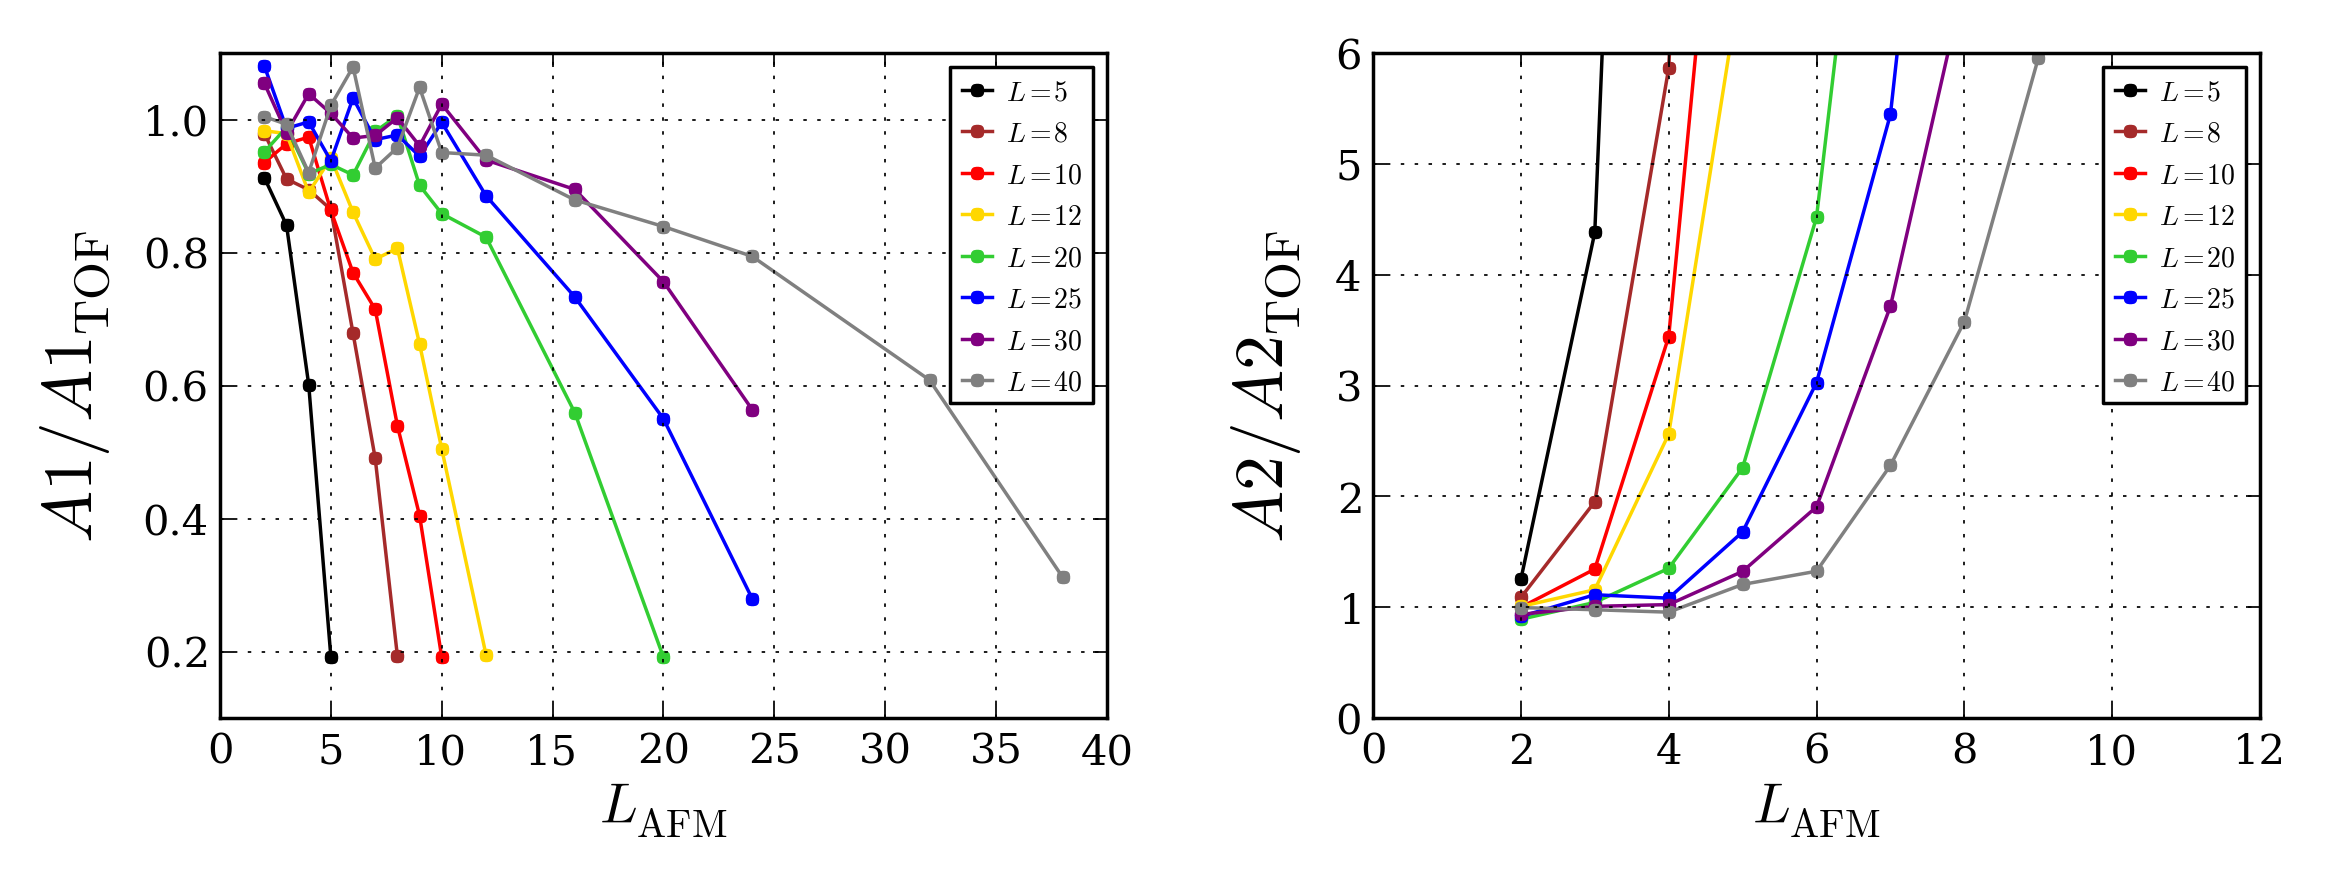
\includegraphics[width=\textwidth]{../crystalsize/CrystalSize.png}
\caption[Bragg for different system sizes]{\small Left panel shows the intensity at camera $A1$ normalized to TOF for different system sizes and AFM core sizes.  Right panel shows the same for the $A2$ camera. }
\label{fig:braggCrystalSize}
\end{figure}
   Our system size is approximately $L=40$,  and
for this size the Bragg signals that we obtain $A2_{\mathrm{t}}\approx1.25$ (we
have seen up to 1.5 sometimes) would be consistent with an AFM core size of
approximately $6^{3}$ sites.  On the other hand we also see a depletion on camera $A1$ of $A1_{t}\approx0.75$, which would be consistent with an AFM core of $25^{3}$ lattice sites.   We believe that our model is not really good for this kind of estimates and this is more the realm of the QMC people, in any case we show what we obtain.  

\subsection{Data with Debye-Waller factor correction for direct comparison with QMC} 
As was mentioned above, our QMC collaborators compute $S(\bv{Q})$, which is related to our measurement as 
\begin{equation}
 I_{t} = 1 +  e^{-2W}( S(\bv{Q}) - 1 )
\end{equation}
where we use the abbreviation $I_{t} = \frac{I}{I_{\mathrm{TOF}}}$.  Previously
we presented our collaborators the data  which did not have a Debye-Waller
factor correction.   Here we make a correction, also noting that we only made
measurements in-situ, $T=0$,  and at $T=6$~$\mu$s TOF.   With these two measurements one can
solve for the spin structure factor 
\begin{equation}
\begin{split}
    A = & \,\,\mathrm{constant }\\
 I_{0} = &A( 1 +  DW_{0}( S(\bv{Q}) - 1 ) ) \\
 I_{T} = &A( 1 +  DW_{T}( S(\bv{Q}) - 1 ) ) \\
 I_{t} \equiv \frac{ I_{0}}{I_{T}} =& \frac{ 1 + DW_{0}(S(\bv{Q})-1) }{ 1 + DW_{T}(S(\bv{Q})-1)} \\
\Rightarrow S(\bv{Q}) =& \frac{  I_{t}(1-DW_{T}) - (1-DW_{0})}{ DW_{0} - I_{t}DW_{T} }\end{split} 
\end{equation}
The data including this Debye-Waller factor correction is shown in Fig.~\ref{fig:data}.
\begin{figure}
\centering 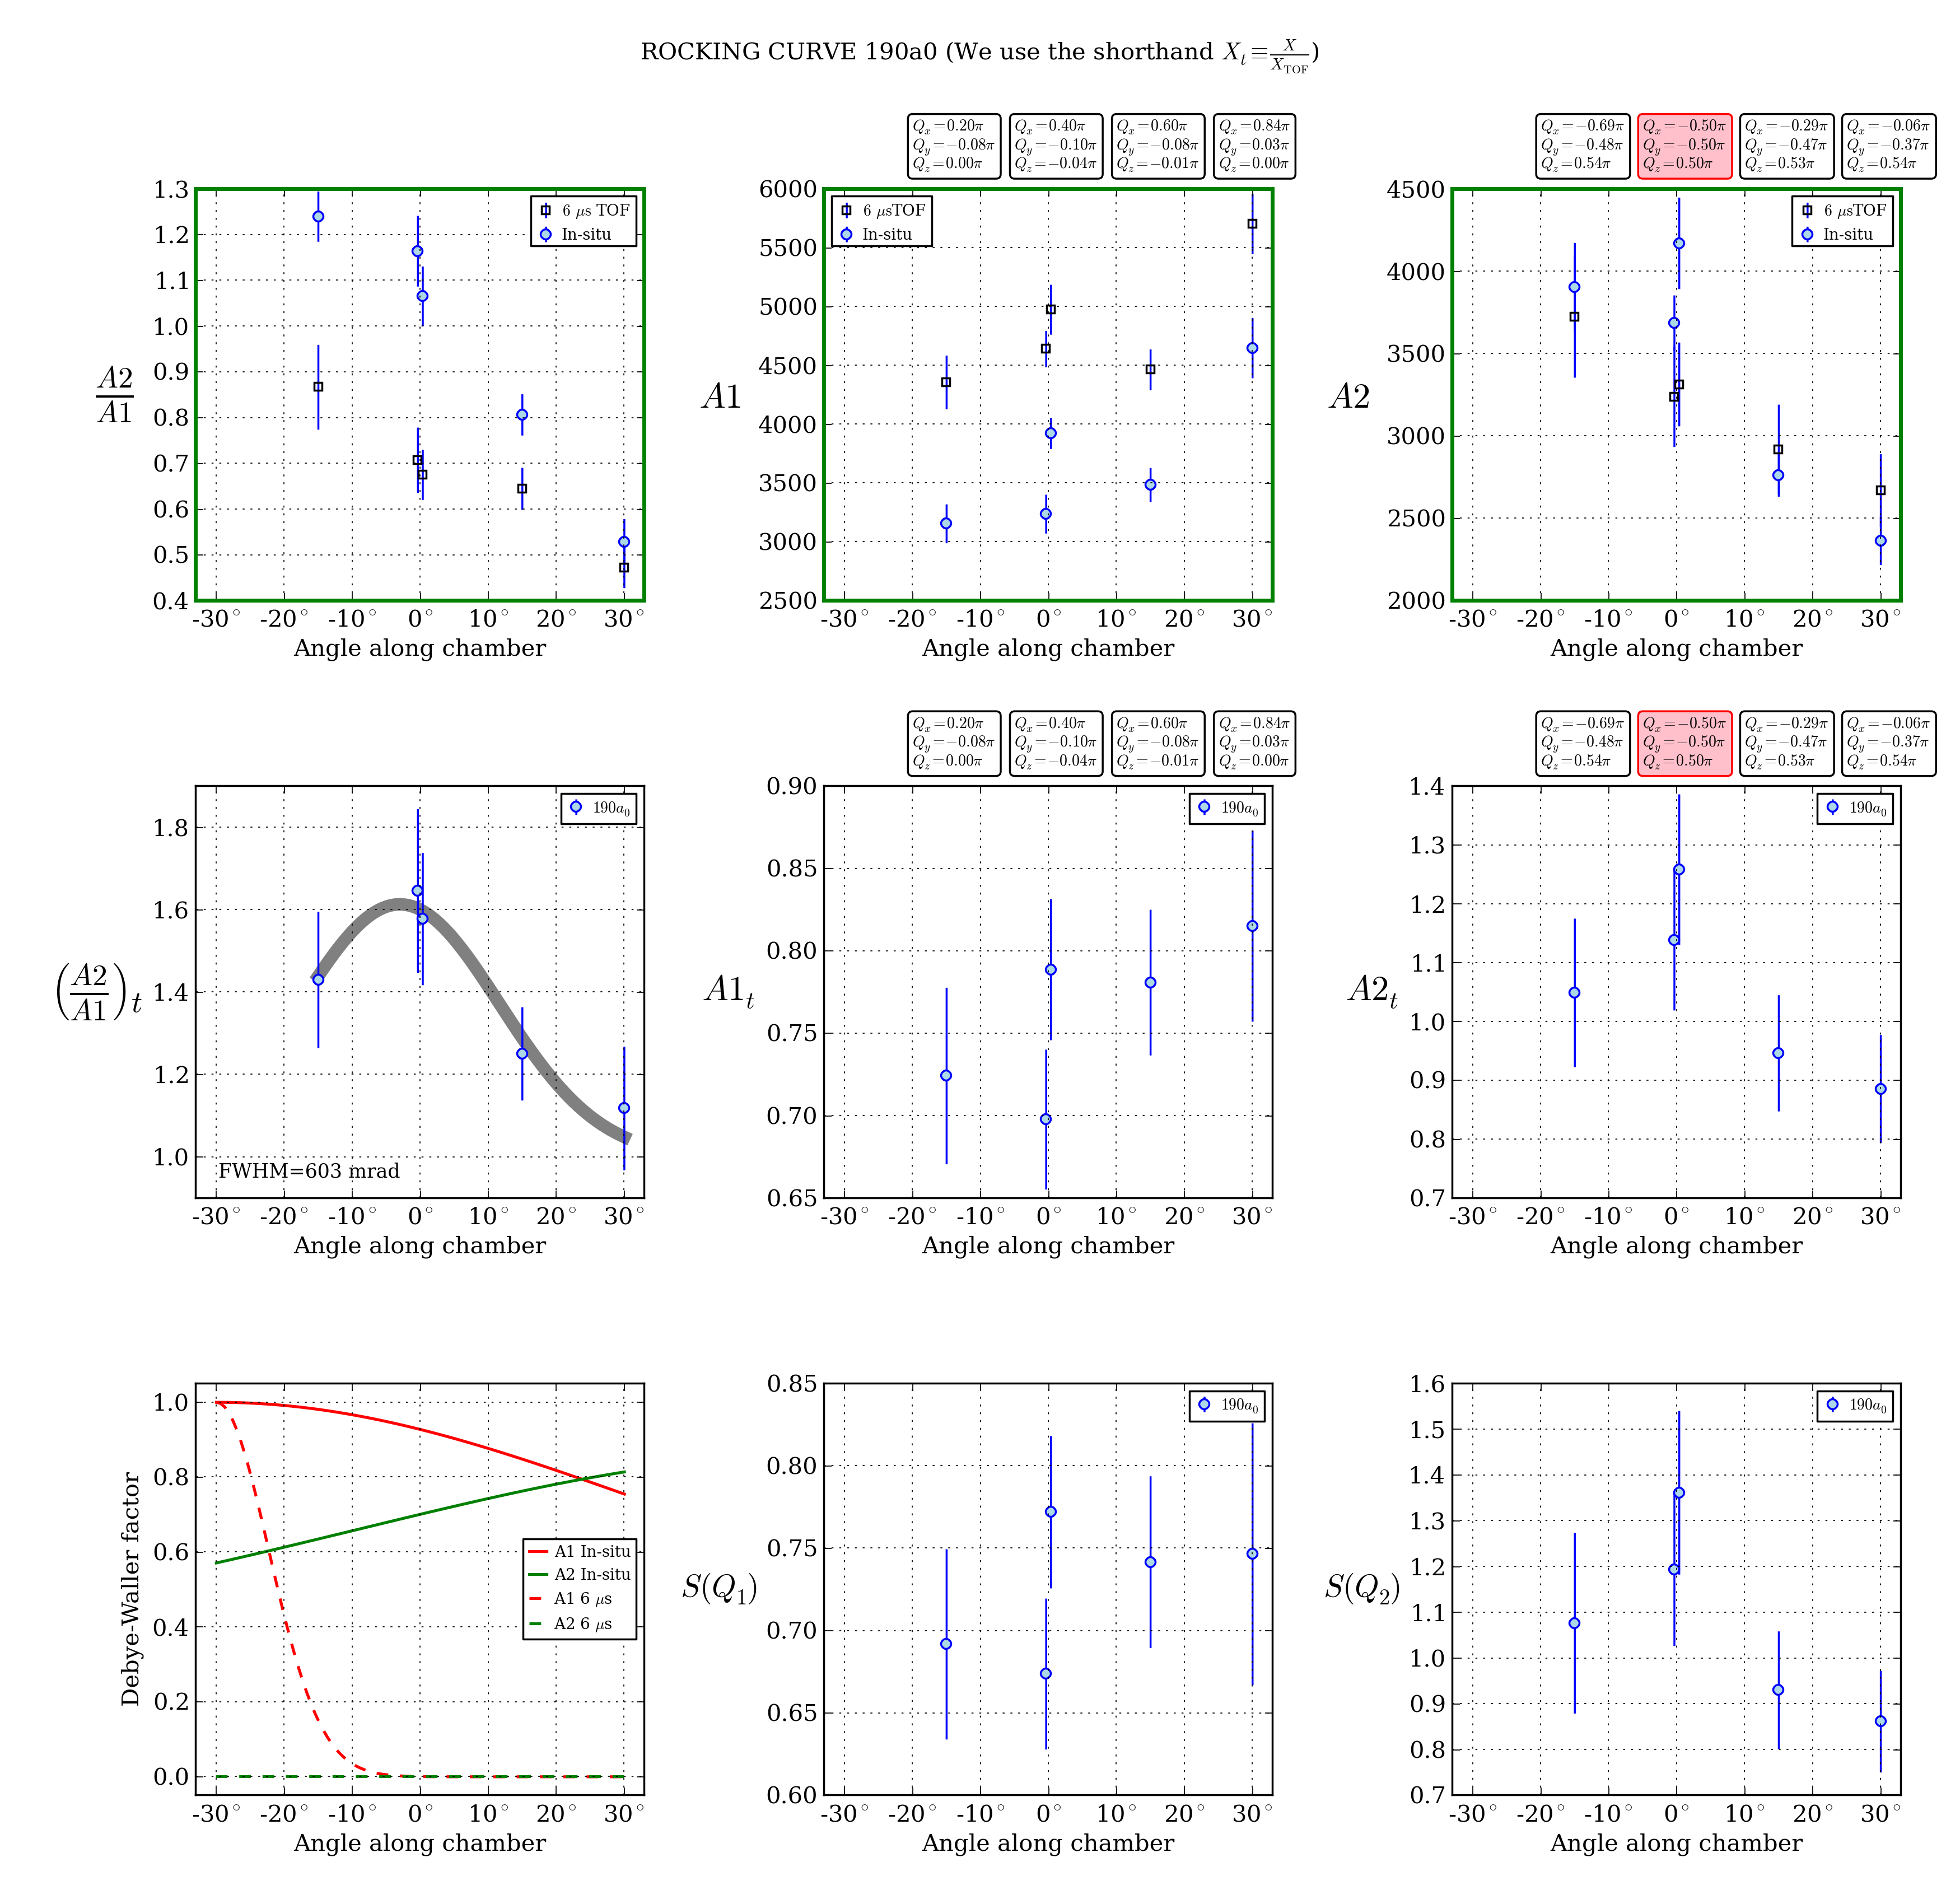
\includegraphics[width=\textwidth]{figures/rocking.png}
\caption[Rocking at 190$a_{0}$]{\small Top row shows our raw data, which corresponds to ratio of CCD counts $A2/A1$, and CCD counts for $A1$, $A2$ respectively.  Middle row shows the ratio of in-situ and TOF data for each of the three quantities.  Bottom row, left panel shows the Debye-Waller factor for the in-situ picture and the 6~$\mu$s TOF picture as a function of angle along chamber.  The $A1$ Debye-Waller factor goes to 1 for both in-situ and TOF at 30$^{\circ}$, which corresponds to zero momentum transfer.  Bottom row, right panels show the spin structure factor determined from our data and the Debye-Waller factor corrections. }
\label{fig:data}
\end{figure}


 
%\subsection{ Analytical dependence of crystal and magnetic structure factors
%on \bv{Q}}
%
%\subsubsection{Crystal}
%
%\begin{equation}
%C(\bv{Q}) = \sum_{jk} e^{i \bv{Q} \cdot (\bv{R}_{j} - \bv{R}_{k} )} 
%\end{equation}
%
%We can make the substitution $\bv{r}_{k} = \bv{R}_{j} -
%\bv{R}_{k}$.  For an infinite crystal, the sum over all pairs $jk$ may be replaced by the sum over all
%sites $j$ and then sum over all $\bv{r}_{k}$.
% 
%\begin{equation}
%C(\bv{Q}) = N\sum_{k} e^{i \bv{Q} \cdot \bv{r}_{k}} 
%\end{equation}
%
%\subsubsection{Magnetic}
%
%\begin{equation}
%S(\bv{Q}) = \sum_{jk} e^{i \bv{Q} \cdot (\bv{R}_{j} - \bv{R}_{k} )} \langle S_{zj} S_{zk} \rangle
%\end{equation}
%
%In the zero temperature AFM state there is a staggered magnetization, such that 
%
%\begin{equation}
%\langle S_{zj}S_{zk} \rangle = e^{i \bv{q} \cdot (\bv{R}_{j} - \bv{R}_{k} )} 
%\ \ \ \mathrm{where} \ \ \  
%\bv{q} = \frac{2\pi}{a} \left( \frac{1}{2}\, \frac{1}{2}\, \frac{1}{2} \right)
%\end{equation}
%
%At finite temperature, the staggered magnetization will have a finite correlation length \Lc, which results in 
%
%\begin{equation}
%\langle S_{zj}S_{zk} \rangle = e^{i \bv{q} \cdot (\bv{R}_{j} - \bv{R}_{k} )} e^{-|\bv{R}_{j} -\bv{R}_{k} |/ \Lc }
% \ \ \ \mathrm{where} \ \ \   
%\bv{q} = \frac{2\pi}{a} \left( \frac{1}{2}\, \frac{1}{2}\, \frac{1}{2} \right)
%\end{equation}
%
%\begin{equation}
%S(\bv{Q}) = \sum_{jk} e^{i (\bv{Q} + \bv{q} )\cdot (\bv{R}_{j} - \bv{R}_{k} )} e^{-|\bv{R}_{j} -\bv{R}_{k} |/ \Lc }
%\end{equation}
%
%At this point we can make the substitution $\bv{r}_{k} = \bv{R}_{j} -
%\bv{R}_{k}$.  For an infinite crystal, the sum over all pairs $jk$ may be replaced by the sum over all
%sites $j$ and then sum over all $\bv{r}_{k}$. 
%
%\begin{equation}
%S(\bv{Q}) = \sum_{jk} e^{i (\bv{Q} + \bv{q} )\cdot \bv{r}_{k} } e^{-r_{k}/ \Lc } = N \sum_{k} e^{i (\bv{Q} + \bv{q} )\cdot \bv{r}_{k} } e^{-r_{k}/ \Lc }
%\end{equation}

\bibliographystyle{osa}
\bibliography{bragg}

\end{document}




